\documentclass[letterpaper]{article} 
\usepackage[left = 0.5in, right = 0.5in, top = 0.9in, bottom = 0.9in]{geometry}
\usepackage{enumitem}
\usepackage{multicol}
\usepackage[spanish]{babel}
\usepackage[utf8]{inputenc}

\usepackage{amsmath,amssymb,amsthm}
\usepackage{tikz-cd}
\usepackage{mathrsfs}
\usepackage[bbgreekl]{mathbbol}
\usepackage{dsfont}
\usepackage{graphicx}
\graphicspath{{img/}}

\newcommand{\op}{\operatorname}
\newcommand{\Op}{^{\op{op}}}
\newcommand{\scc}{\mathscr C}
\newcommand{\scd}{\mathscr D}
\newcommand{\sce}{\mathscr E}
\newcommand{\sci}{\mathscr I}
\newcommand{\scj}{\mathscr J}
\newcommand{\scx}{\mathscr X}
\newcommand{\var}{\mathrm{Var}}
\newcommand{\Id}{\operatorname{Id}}
\newcommand{\N}{\mathbb N}
\newcommand{\Z}{\mathbb Z}
\newcommand{\Q}{\mathbb{Q}}
\newcommand{\I}{\mathbb{I}}
\newcommand{\R}{\mathbb{R}}
\newcommand{\C}{\mathbb{C}}
\newcommand{\F}{\mathcal{F}}
\newcommand{\G}{\mathcal{G}}
\newcommand{\B}{\mathcal{B}}
\newcommand{\abs}[1]{\left\lvert #1 \right\rvert}
\newcommand{\inv}{^{-1}}
\renewcommand{\to}{\rightarrow}
\newcommand{\ent}{\Longrightarrow}
\newcommand{\E}{\mathbb{E}}
\renewcommand{\P}{\mathbb{P}}
\newcommand{\1}{\mathds{1}}
\renewcommand{\qedsymbol}{$\blacksquare$}

\theoremstyle{definition}
\newtheorem{dfn}{Definición}
\theoremstyle{definition}
\newtheorem{teo}{Teorema}
\theoremstyle{definition}
\newtheorem{cor}{Corolario}
\theoremstyle{definition}
\newtheorem{prop}{Proposición}
\theoremstyle{definition}
\newtheorem{obs}{Observación}


\title{\textbf{Cómputo Científico\\
Tarea 7\\
MCMC: Metrópolis-Hastings II}}
\author{Iván Irving Rosas Domínguez}
\date{\today}

\DeclareSymbolFontAlphabet{\mathbbm}{bbold}
\DeclareSymbolFontAlphabet{\mathbb}{AMSb}
\DeclareMathSymbol\bbDelta  \mathord{bbold}{"01}

\begin{document}
\maketitle

% \begin{abstract}
% \end{abstract}

\textbf{Con el algoritmo Metrópolis-Hastings (MH), simular lo siguiente, contemplando que en cada ejercicio:}
\begin{itemize}
    \item Establece cual es tu distribución inicial.
    \item Grafica la evolución de la cadena.
    \item Indica cuál es el Burn-in.
    \item Comenta qué tan eficiente es la cadena.
    \item Implementa el algoritmo MH considerando una propuesta diferente.
\end{itemize}
Todos los ejercicios de esta tarea se encuentran en el script \textit{Cómputo Tarea 7} divididos con comentarios.
Asimismo, la semilla utilizada para todos los resultados está dada por $np.random.seed(10)$. Por motivo de brevedad en este 
documento los detalles sobre la implementación de las funciones se encuentran en los comentarios del código.
\section*{Ejercicio 1:}
Sean $x_i\sim\Gamma(\alpha,\beta); \ i\in \{1,...,n\}$. Simular datos $x_i$ 
con $\alpha=3$ y $\beta=100$ considerando los casos $n=4$ y $n=30$.

Con $\alpha\sim U(1,4)$, $\beta\sim \exp(1)$ distribuciones a priori, se tiene la
posterior 
\[
f(\alpha,\beta|\bar{x})\propto\frac{\beta^{n\alpha}}{\Gamma^{n}(\alpha)}r_1^{\alpha-1}e^{-\beta(r_2+1)}, \qquad 1\leq \alpha\leq 4, \quad \beta>0.    
\]

con $r_2=\displaystyle \sum_{i=1}^nx_i$ y $r_1=\displaystyle\prod_{i=1}^{n}x_i$.

En ambos casos, grafica los contornos para visualizar dónde está concentrada la posterior.

Utilizar la propuesta 
\[
q \left( \begin{pmatrix}
    \alpha_p\\
    \beta_p
\end{pmatrix} \Bigg|
\begin{pmatrix}
    \alpha\\
    \beta
\end{pmatrix}
\right)= \begin{pmatrix}
    \alpha\\
    \beta
\end{pmatrix}
+
\begin{pmatrix}
    \varepsilon_1\\
    \varepsilon_2
\end{pmatrix},    
\]
donde 
\[
\begin{pmatrix}
    \varepsilon_1\\
    \varepsilon_2
\end{pmatrix}    
\sim 
\mathcal{N}_2 \left( \begin{pmatrix}
    0\\
    0
\end{pmatrix},
\begin{pmatrix}
    \sigma_1^2 & 0\\
    0 & \sigma_2^2
\end{pmatrix}\right).
\]
\subsection*{Solución:}

Para el análisis de esta implementación, así como del resto de los incisos, se construyeron las funciones respectivas para evaluar dos puntos en la 
posterior, para calcular el cociente de MH y para realizar el algoritmo mismo. Dichas funciones tienen 
la particularidad de poder cambiar entre la propuesta 1, que contiene la implementación correspondiente al ejercicio en cuestión 
de la tarea, y la propuesta 2, que contiene la implementación diferente. La implementación del algoritmo utilizando una propuesta diferente se difiere siempre hasta el final de los incisos.\\

Dicho lo anterior, comenzamos este ejercicio separando los casos $n=4$ y $n=30$
\subsubsection*{Caso n=4}
En este caso, se simulan primero 4 datos $X_1,...,X_4$ con distribuciones $\Gamma(3,100)$. Se guardan 
las sumas y los productos tal y como indica el ejercicio, y se implementa el algoritmo. Se obtienen los siguientes resultados:

\begin{figure}[h!]
    \centering
    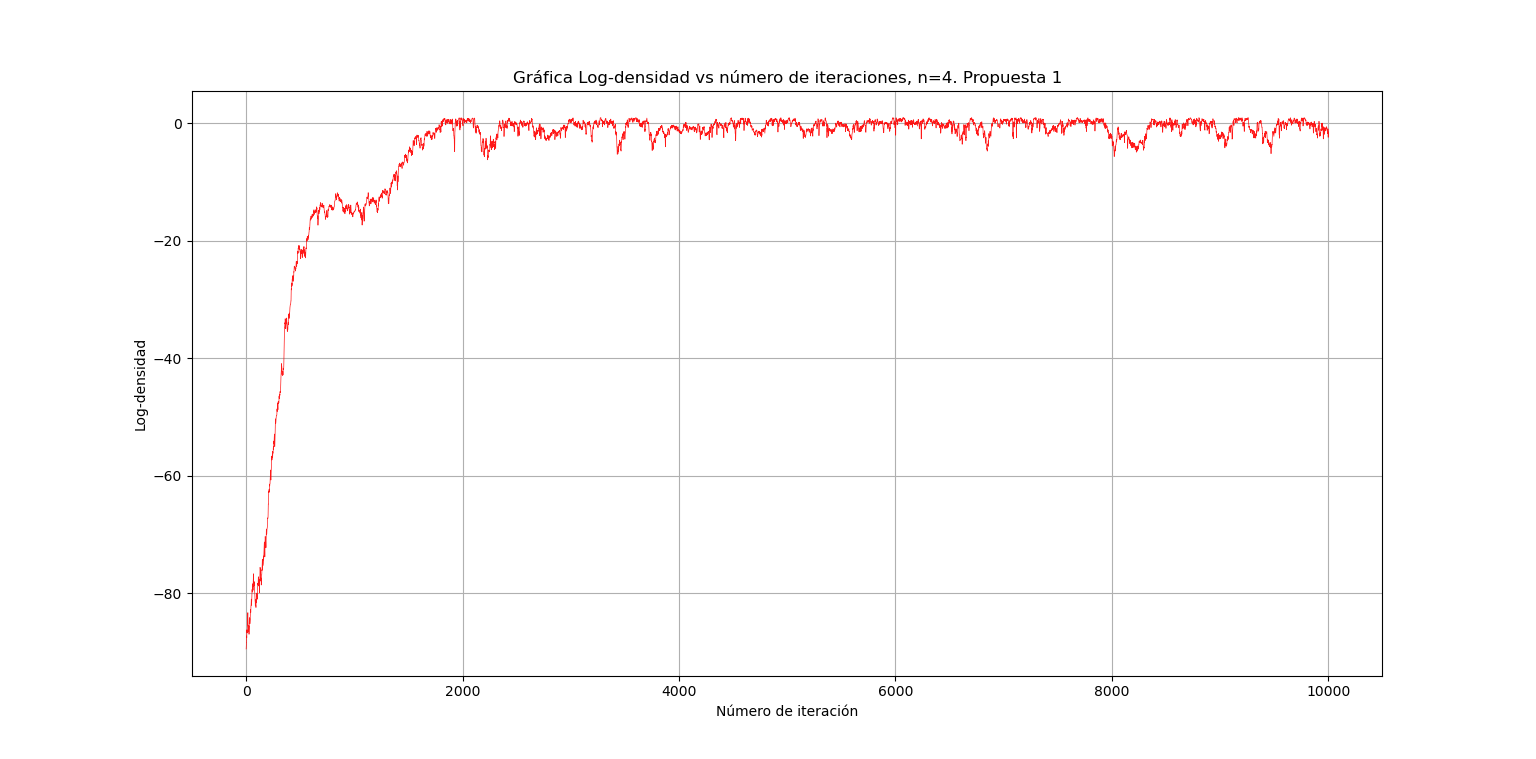
\includegraphics[width=\linewidth]{1.png}
    \caption{}
\end{figure} 
\begin{figure}[h!]
    \centering
    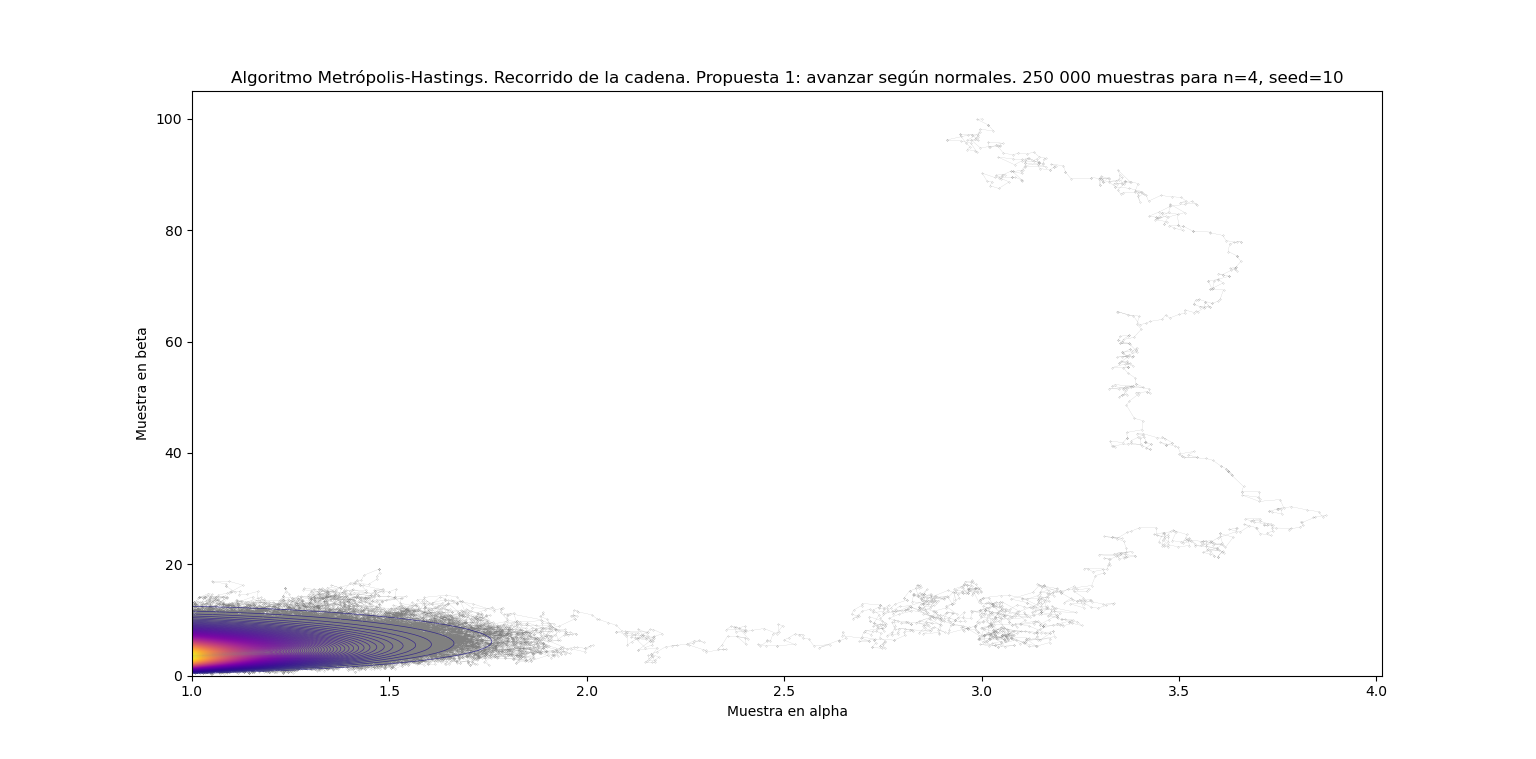
\includegraphics[width=\linewidth]{2.png}
    \caption{}
\end{figure} 
\begin{figure}[h!]
    \centering
    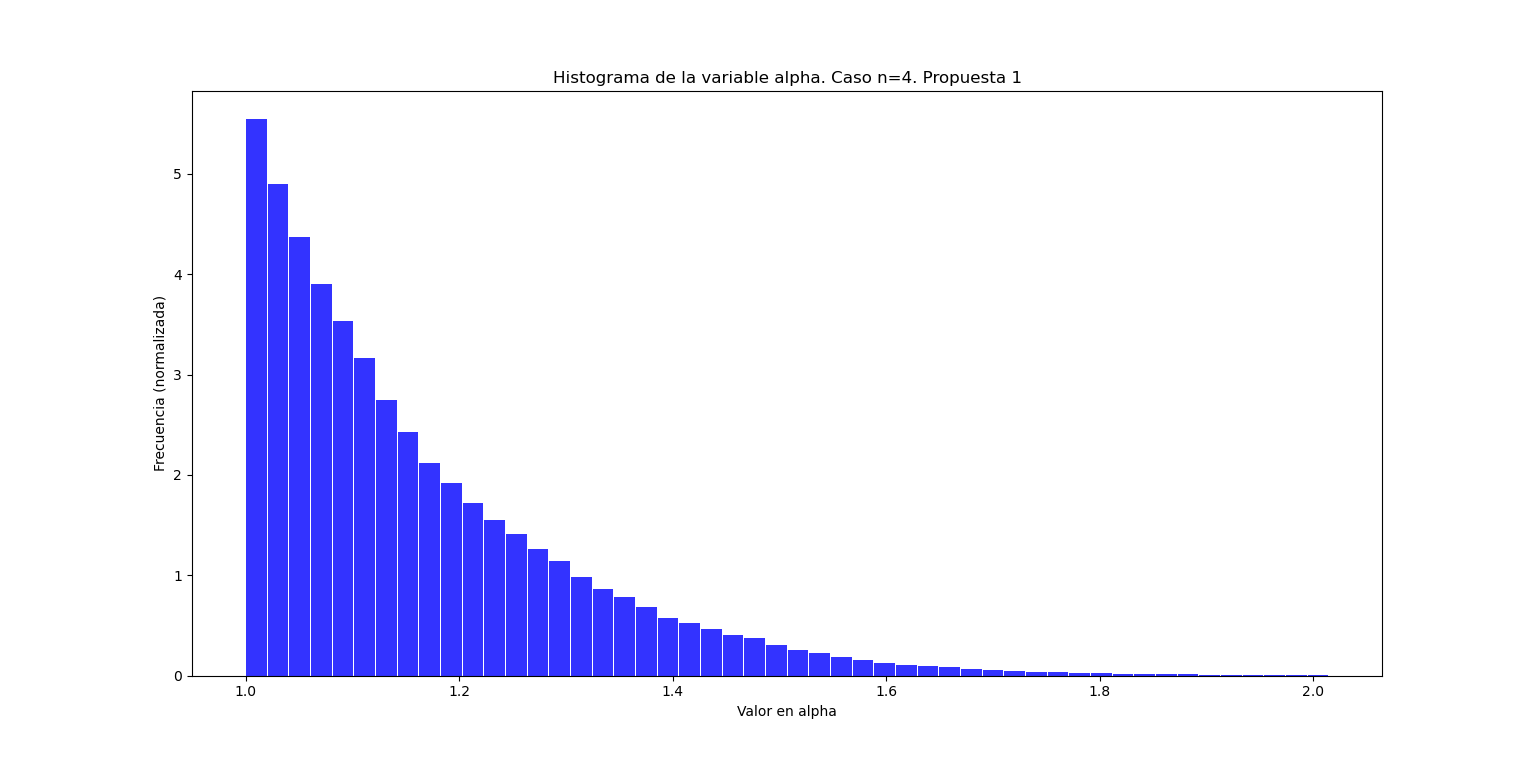
\includegraphics[width=\linewidth]{3.png}
    \caption{}
\end{figure} 
\begin{figure}[h!]
    \centering
    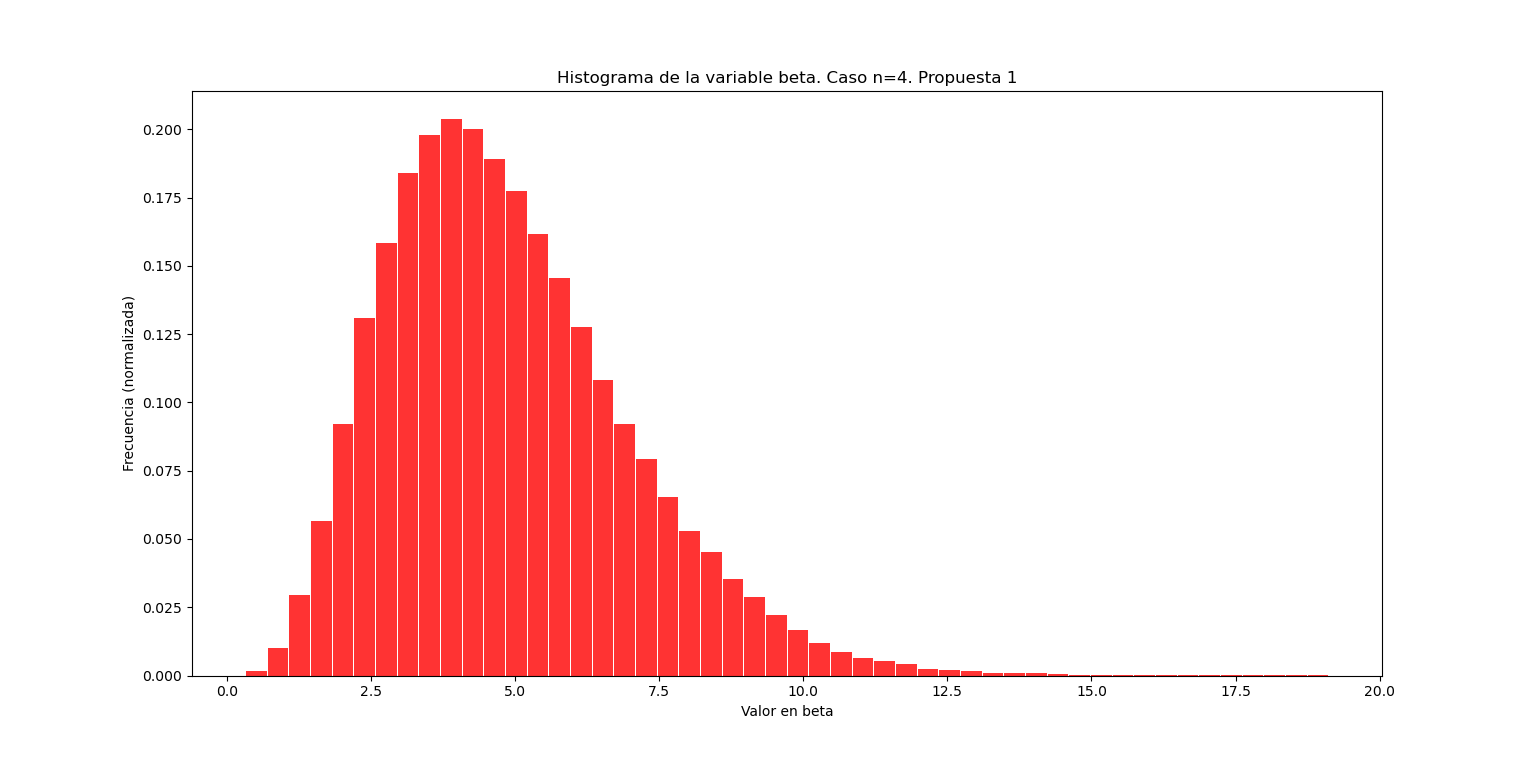
\includegraphics[width=\linewidth]{4.png}
    \caption{}
\end{figure} 

En particular de la figura 1 se puede deducir que un burn-in adecuado ronda $n=3000$. En la figura 2 podemos 
apreciar la convergencia de la cadena hacia la distribución objetivo. Finalmente en las figuras 3 y 4 se aprecian 
las densidades marginales de lo que serían los parámetros a posteriori $\alpha$ y $\beta$. Dichos histogramas ya 
tienen en cuenta el burn-in. A primera vista 
tienen forma de exponenciales y gamma respectivamente.

\subsubsection*{Caso n=30}
Simulamos ahora $X_1,...,X_{30}\sim \Gamma(3,100)$. Nuevamente se implementan las sumas, el producto, y se ejecuta el algoritmo. Los resultados a continuación:
\begin{figure}[h!]
    \centering
    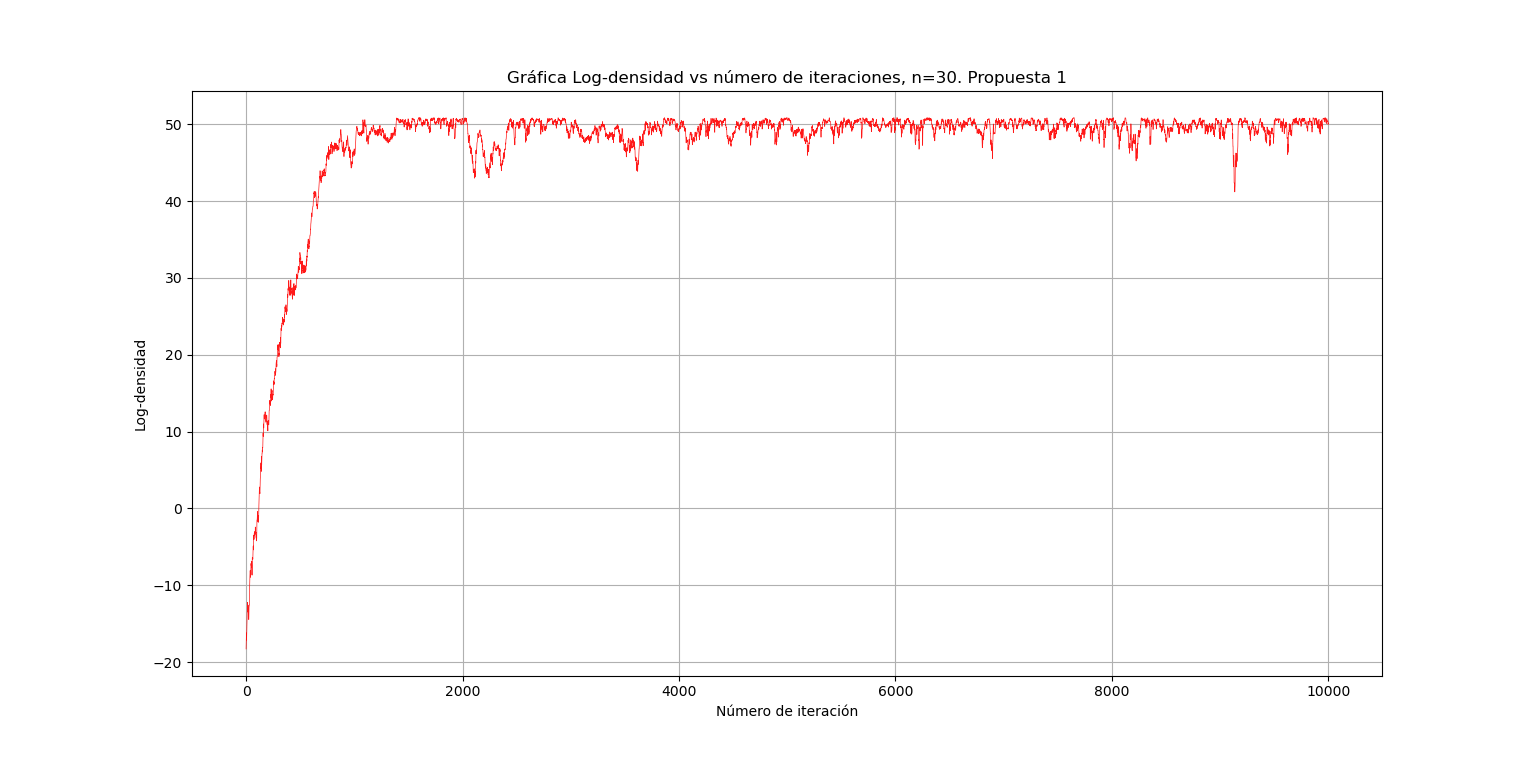
\includegraphics[width=\linewidth]{5.png}
    \caption{}
\end{figure} 
\begin{figure}[h!]
    \centering
    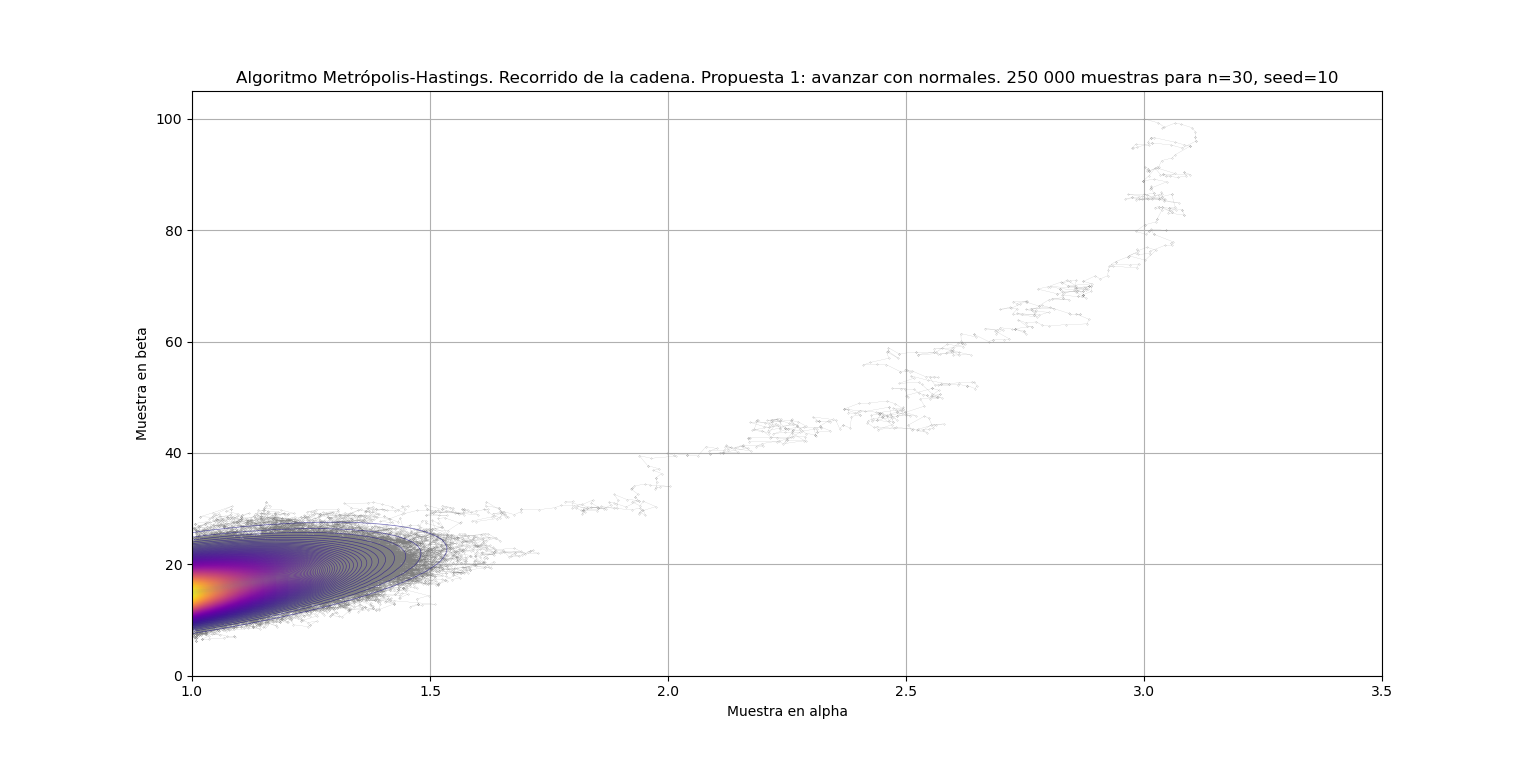
\includegraphics[width=\linewidth]{6.png}
    \caption{}
\end{figure} 
\begin{figure}[h!]
    \centering
    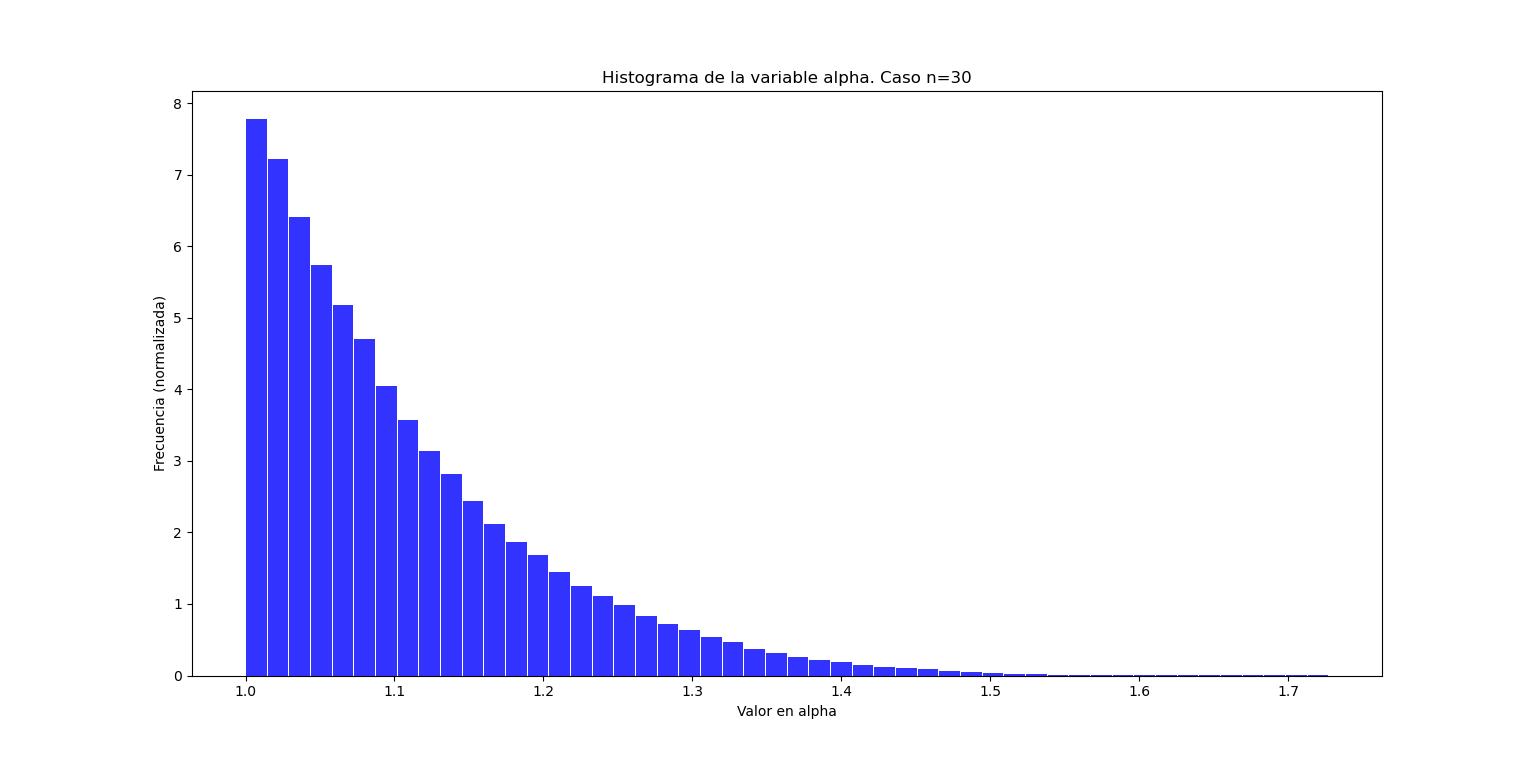
\includegraphics[width=\linewidth]{7.png}
    \caption{}
\end{figure} 
\begin{figure}[h!]
    \centering
    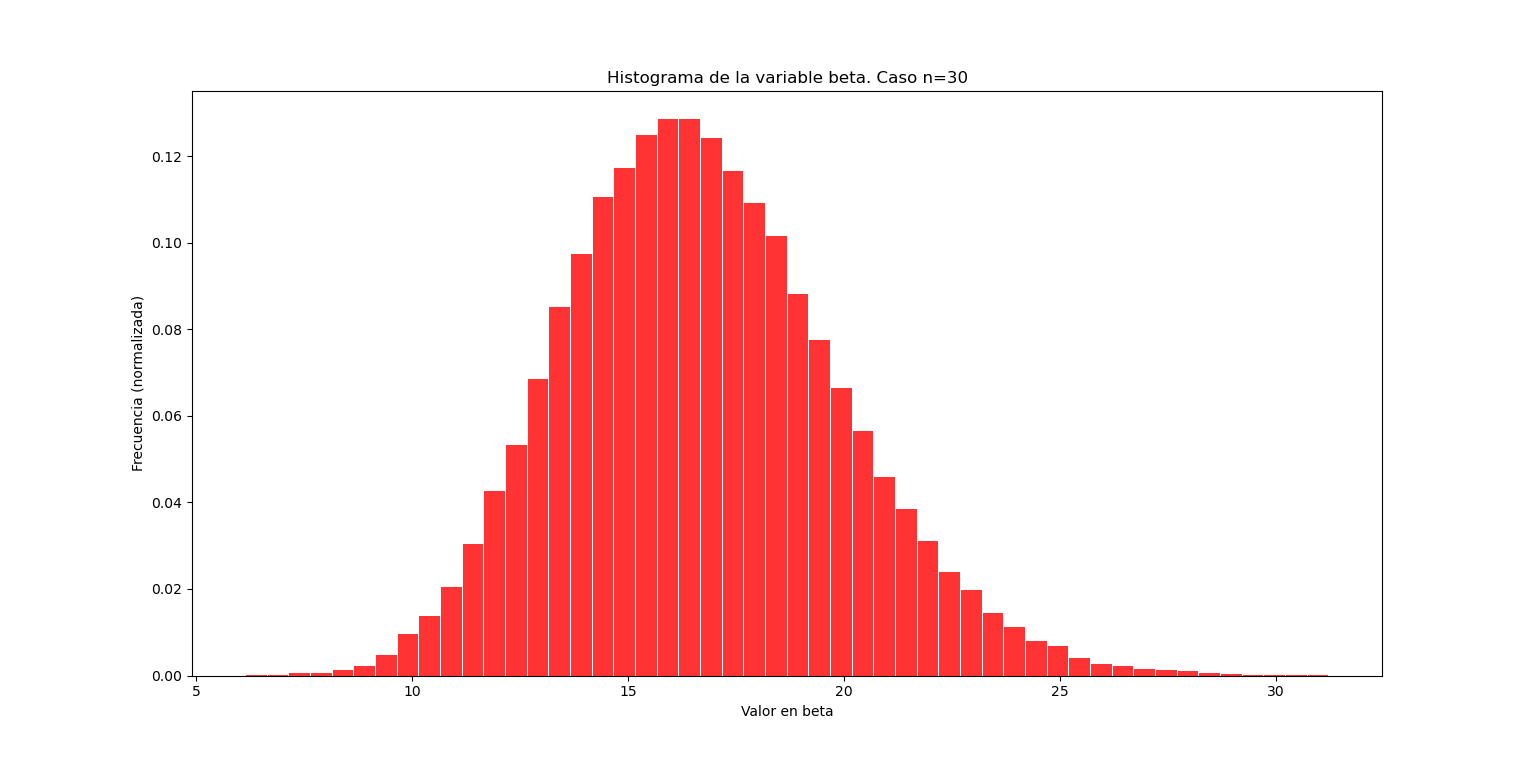
\includegraphics[width=\linewidth]{8.png}
    \caption{}
\end{figure} 
En particular, de la figura 5 nuevamente se puede deducir que un burn-in adecuado ronda la iteración 3000. Luego, tal es 
el valor seleccionado. La figura 6 nos da una idea de la convergencia de la cadena hacia la distribución objetivo. Obesrvamos 
un mejor comportamiento en cuanto a la 'rapidez' a la que la cadena converge. Esto sin duda tiene que ver 
con los parámetros $\sigma_1$ y $\sigma_2$ utilizados en la propuesta. Finalmente, las figuras 7 y 8 son las 
densidades marginales extraídas de las muestras. Ambas nuevamente presentan un comportamiento exponencial y gamma 
respectivamente. Los histogramas ya tienen en cuenta el burn-in.
\newline

Para puntualizar lo dicho antes:
\begin{itemize}
    \item \textbf{Distribución inicial}: tomamos el vector $X_0=(3,100)$ como propuesta. Dicho punto inicial está dentro de las simulaciones $\alpha\sim U(1,4)$ y $\beta\sim exp(1)$
    \item \textbf{Grafica la evolución de la cadena}: ver figuras arriba
    \item \textbf{Burn-in}: para ambos casos, se toma un burn-in=3000. Su justificación está en las figuras anteriormente citadas.
    \item \textbf{¿Qué tan eficiente es la cadena?}: una manera de medir la eficacia de la cadena es observar la gráfica de la log-densidad evaluada en las muestras. Si
     dicha gráfica es tal que se deshace de los valores 'atípicos' en pocas iteraciones, podremos decir que la cadena ha llegado a la distribución objetivo y se mantiene 
    cerca de esta en esas pocas iteraciones, por lo que la cadena es eficiente.\\
    
    En el caso $n=4$, se maneja un burn-in de 3000 justificado en las gráficas de la log-densidad vs el número de iteraciones. Se puede concluir que esta cadena es más
    eficiente que la cadena que utiliza una propuesta diferente (ver debajo). Los parámetros de la cadena están fijados en $\sigma_1=0.0005$ y $\sigma_2=0.5$ respectivamente,
    esto nos indica que se avanza en la variable $\alpha$ (midiendo las cosas en la varianza de la normal propuesta) 1000 veces más en tamaño que lo que se avanza en 
    el parámetro $\beta$. Esto se justifica pues $\beta$ tiene soporte en toda la recta real, mientras que $\alpha$ solo en $(1,4)$.

    \item \textbf{Implementa el algoritmo MH considerando una propuesta diferente.}
    En este caso, se decide implementar la propuesta $y\sim U \left( [-0.03,0.03]x[-0.5,0.5] \right)$.
    Esto es, a cada paso, se simula una uniforme con centro en el punto actual de la cadena, donde 
    la variable uniforme (un cuadradito) tiene de ancho 0.06 y alto 1. Se calcula el cociente 
    de Metrópolis-Hastings y se rechaza o acepta según tal número. Esto nos produce los siguientes resultados.
    Separamos nuevamente los dos casos anteriores. 
\end{itemize}
\subsubsection*{Caso n=4}
Obtenemos los siguientes resultados:
\begin{figure}[h!]
    \centering
    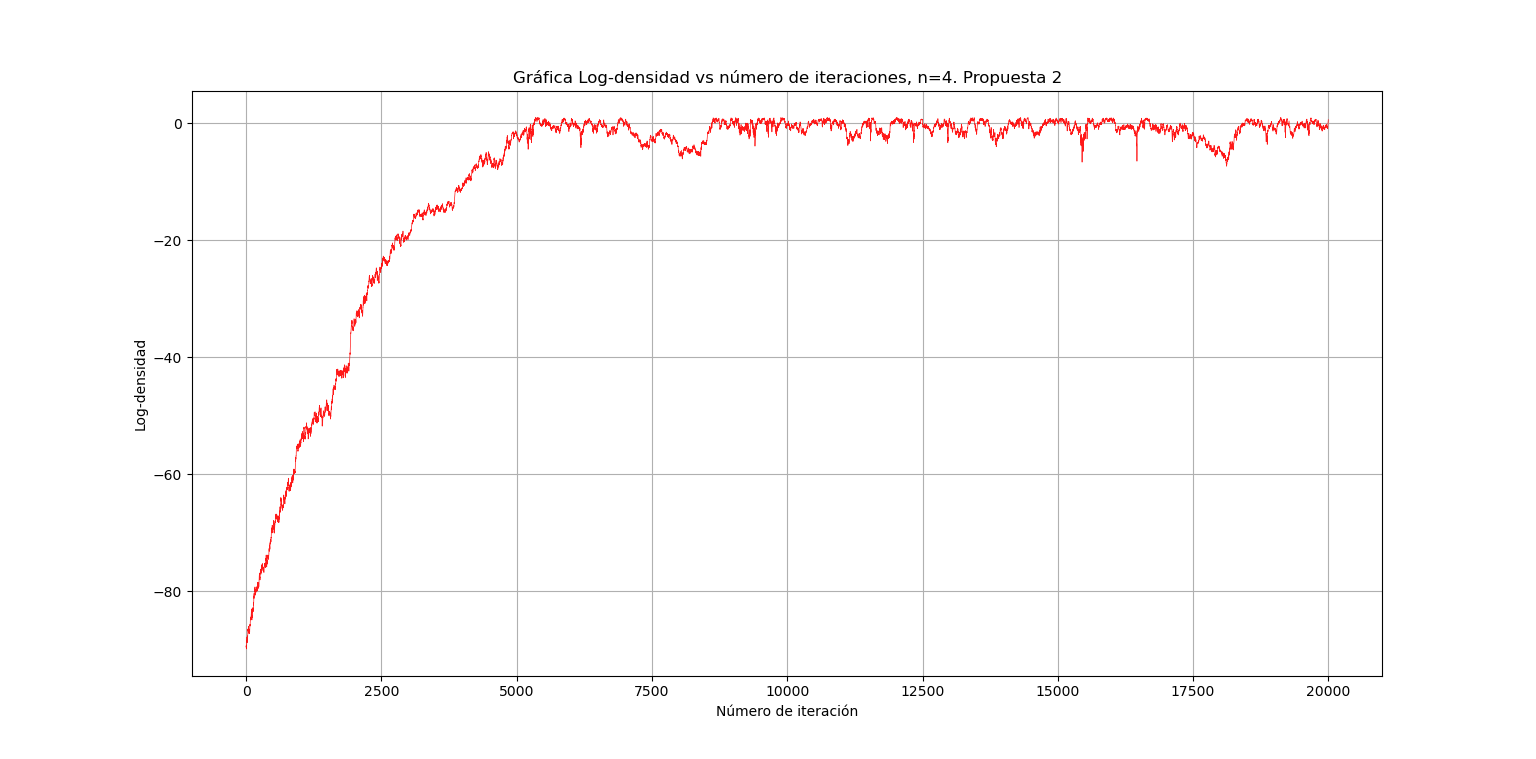
\includegraphics[width=\linewidth]{9.png}
    \caption{}
\end{figure} 
\begin{figure}[h!]
    \centering
    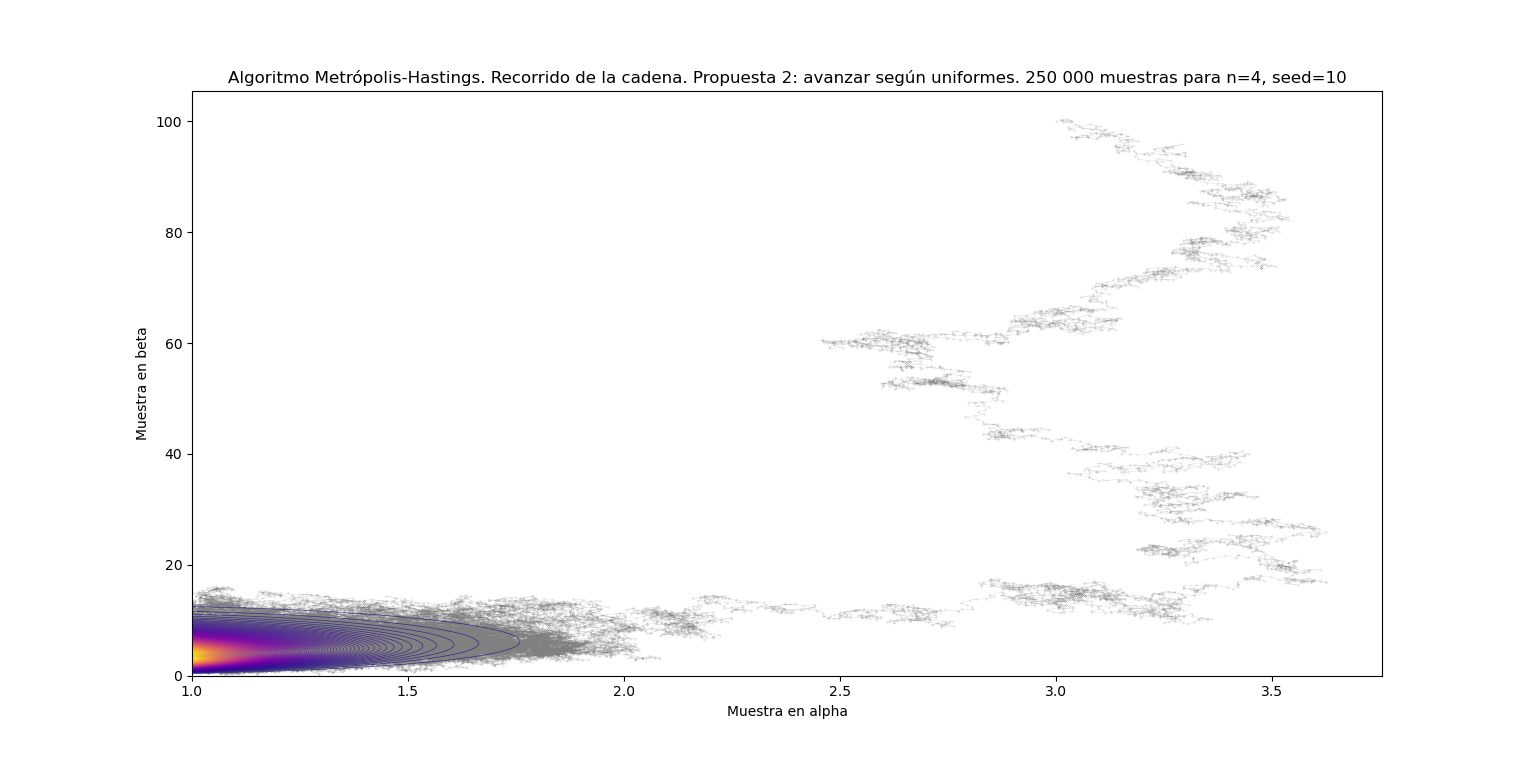
\includegraphics[width=\linewidth]{10.png}
    \caption{}
\end{figure} 
\begin{figure}[h!]
    \centering
    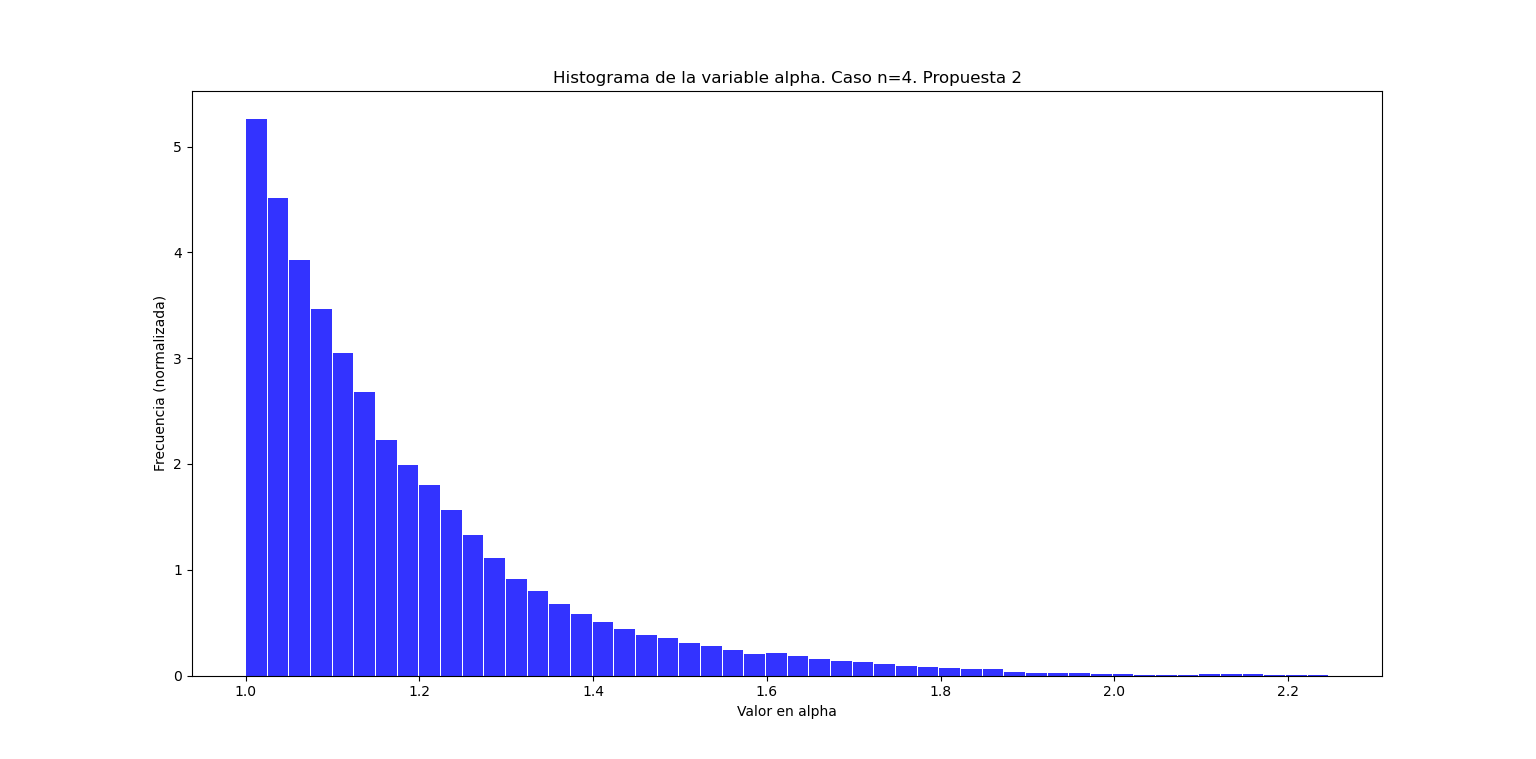
\includegraphics[width=\linewidth]{11.png}
    \caption{}
\end{figure} 
\begin{figure}[h!]
    \centering
    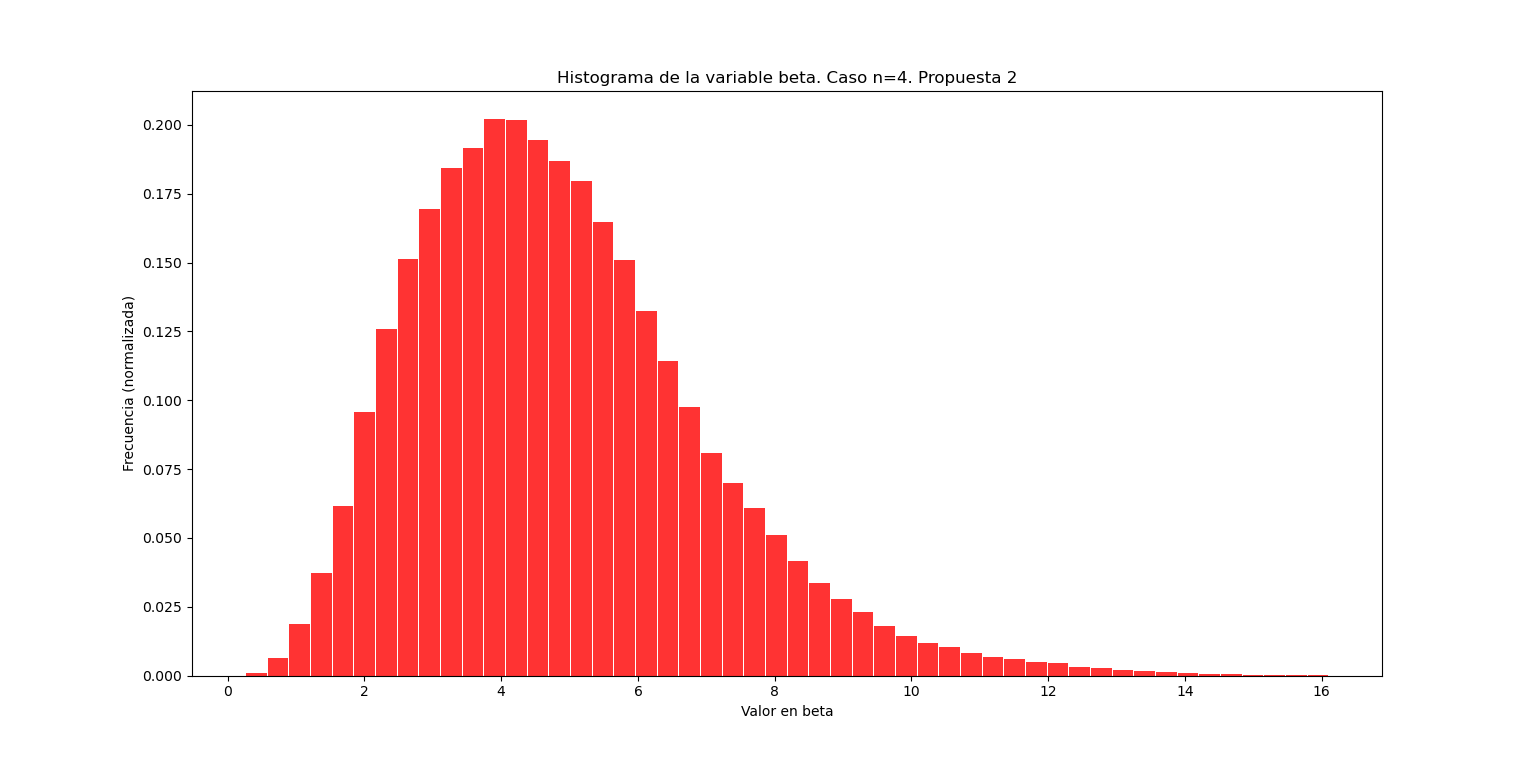
\includegraphics[width=\linewidth]{12.png}
    \caption{}
\end{figure} 
De la figura 9 se puede deducir que un burn-in adecuado ronda la iteración 7000. El avance de la cadena 
se puede ver en la figura 10, mientras que en la figura 11 y 12 se ven los histogramas que aproximan 
las densidades de $\alpha$ y $\beta$. Los histogramas ya contemplan burn-in. Su comportamiento es muy similar a los de las figuras 3 y 4 con la propuesta 1.

\subsubsection*{Caso n=30}
Finalmente tenemos este caso, en donde los resultados son los siguientes:

\begin{figure}[h!]
    \centering
    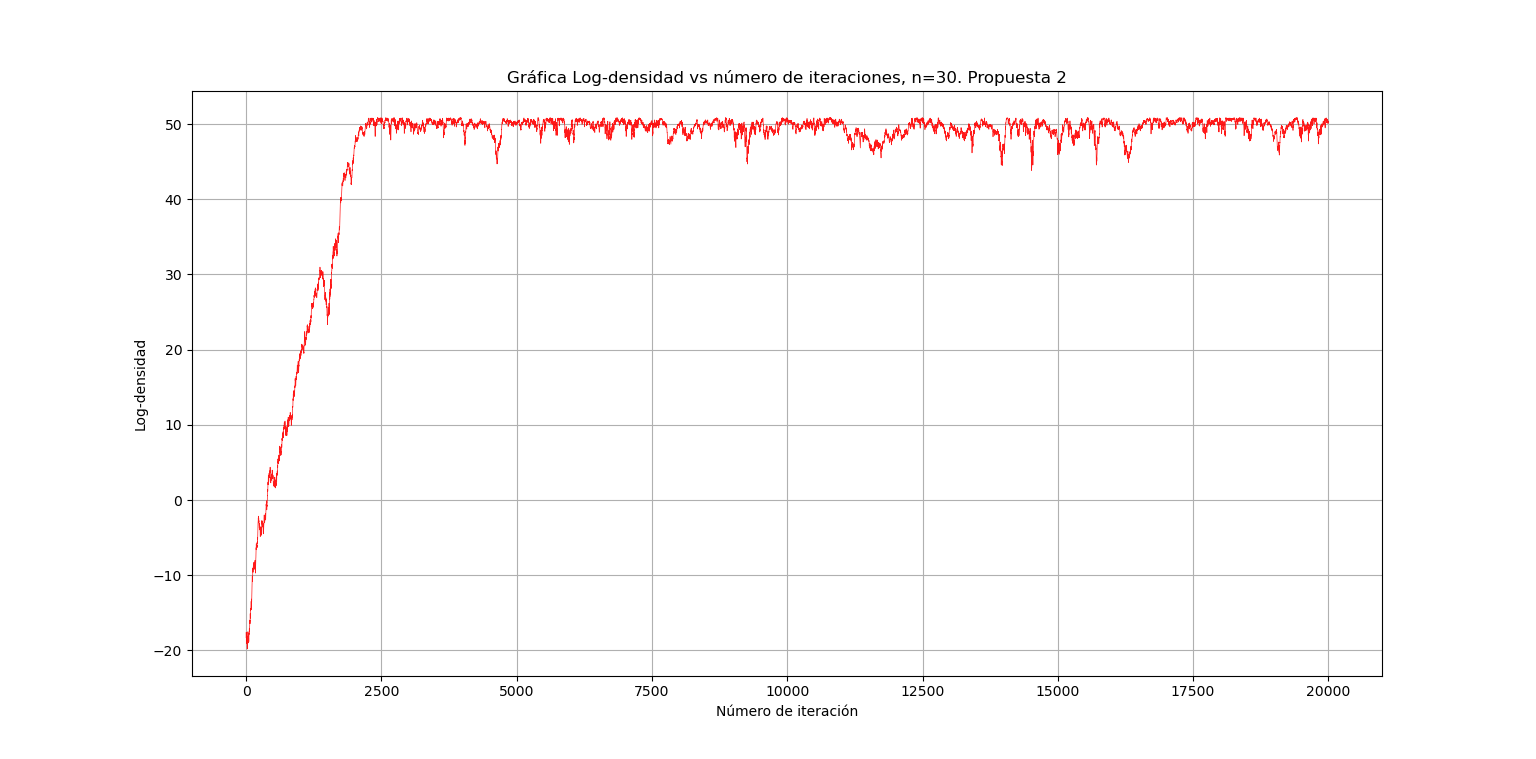
\includegraphics[width=\linewidth]{13.png}
    \caption{}
\end{figure} 
\begin{figure}[h!]
    \centering
    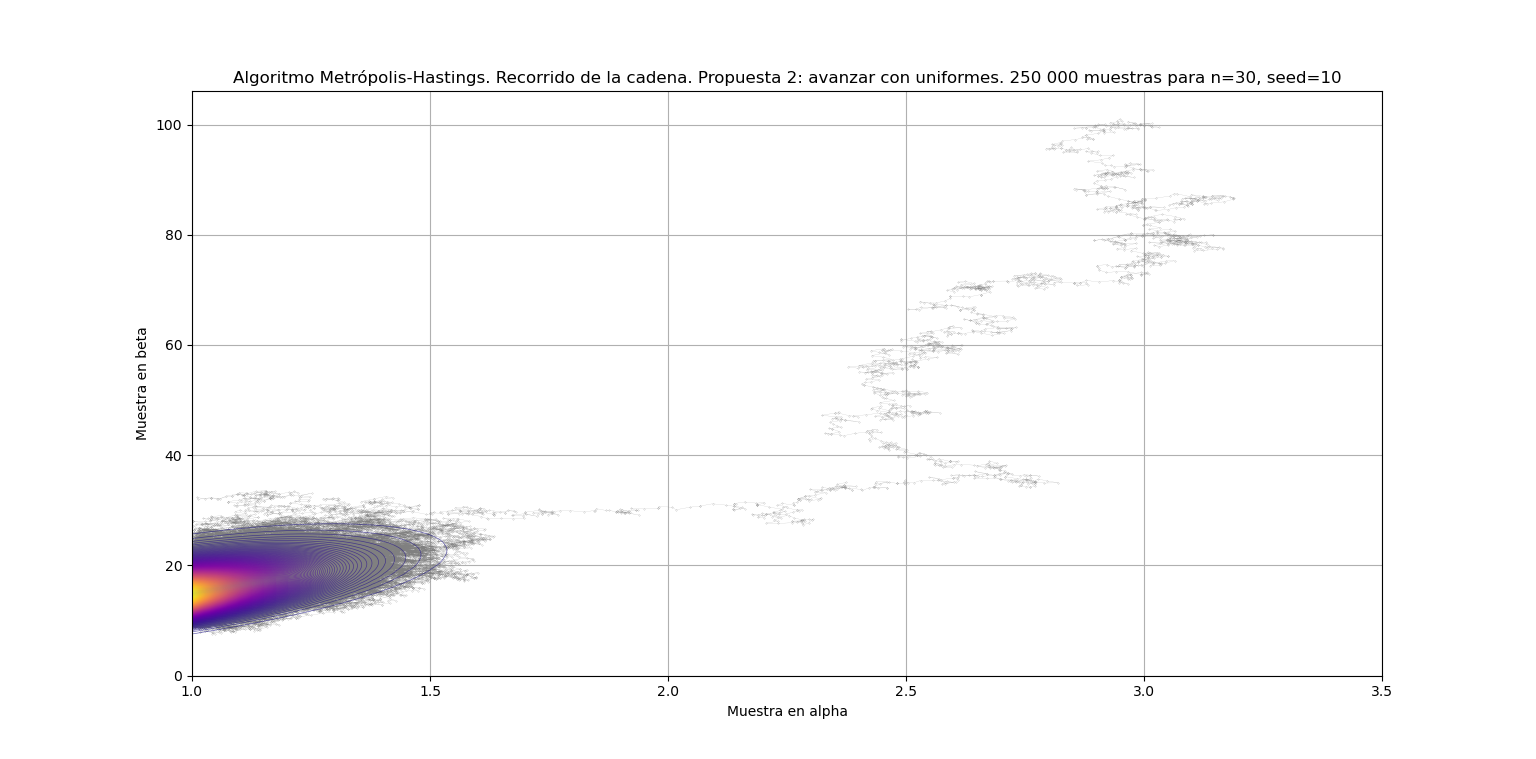
\includegraphics[width=\linewidth]{14.png}
    \caption{}
\end{figure} 
\begin{figure}[h!]
    \centering
    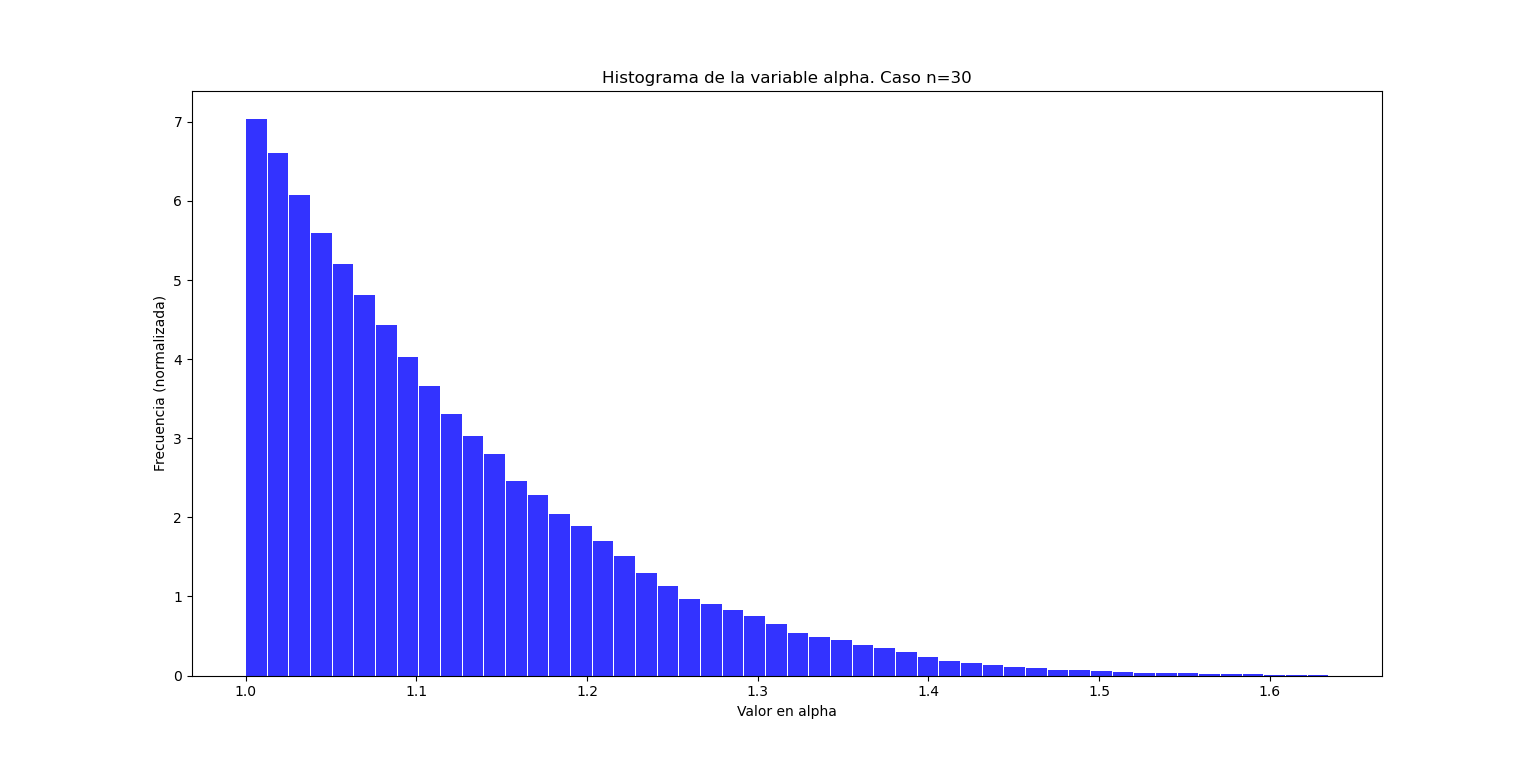
\includegraphics[width=\linewidth]{15.png}
    \caption{}
\end{figure} 
\begin{figure}[h!]
    \centering
    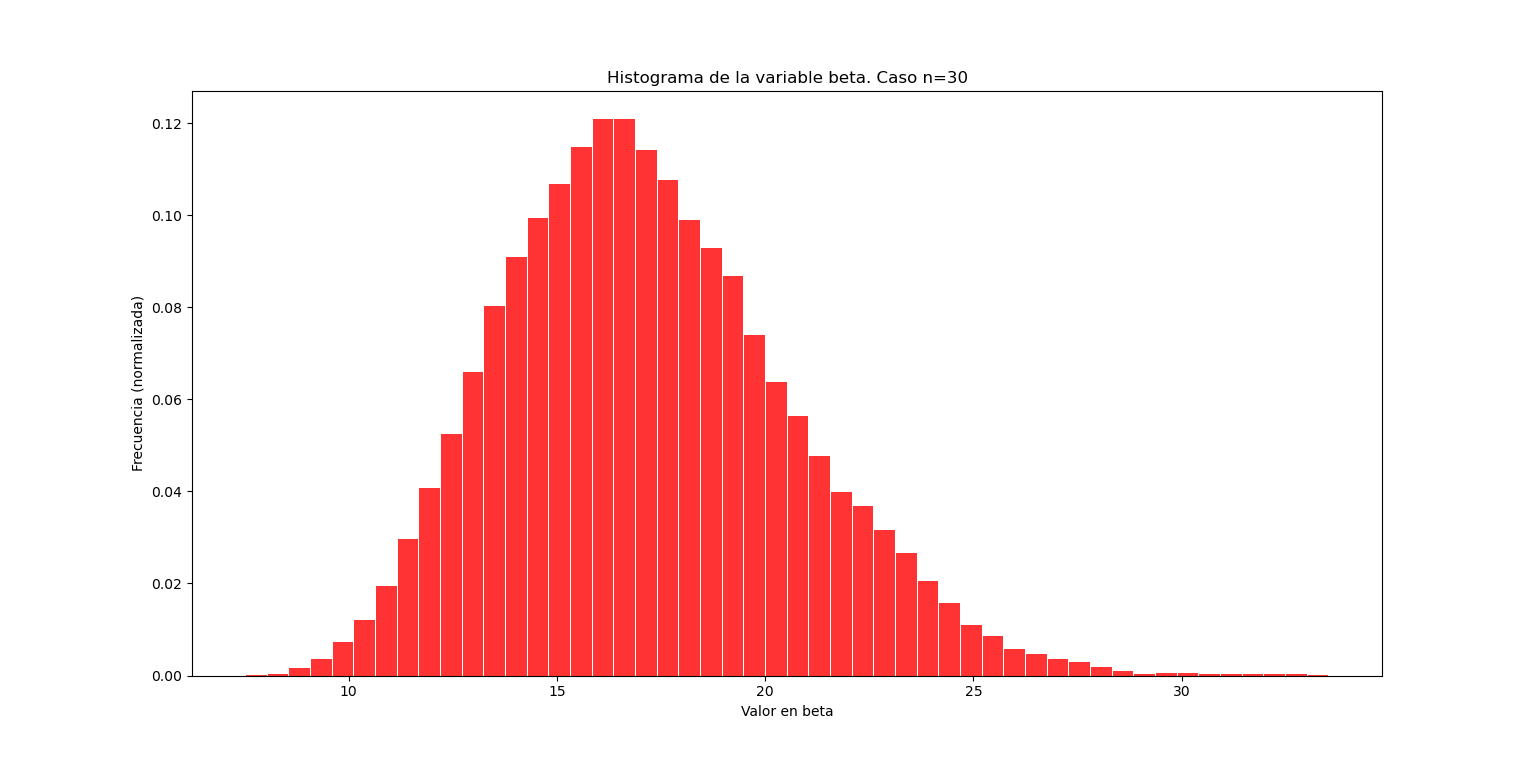
\includegraphics[width=\linewidth]{16.png}
    \caption{}
\end{figure} 
De nueva cuenta en la figura 13 se puede apreciar que un valor adecuado para burn-in es de 7000. 
El recorrido es impreso en la figura 14, mientras que las figuras 15 y 16 muestran los histogramas 
de las densidades marginales. Se puede observar un ligero mejor comportamiento de los histogramas en 
las figuras 7 y 8 que usan la propuesta normal, aún cunado ya se contempla el burn-in en estos.
\\

Para concluir, se detalla lo pedido:

\begin{itemize}
    \item \textbf{Distribución inicial}: tomamos el vector $X_0=(3,100)$ como propuesta inicial nuevamente. 
    \item \textbf{Grafica la evolución de la cadena}: ver figuras arriba.
    \item \textbf{Burn-in}: para ambos casos, se toma un burn-in=7000.
    \item \textbf{¿Qué tan eficiente es la cadena?}: tomando en cuenta el desempeño hecho con la propuesta 1, esta cadena presenta un desempeño 
    menor que el logrado con la otra propuesta. Esto se puede ver también en las gráficas de la log-densidad, donde 
    se está llegando a una 'estabilidad' alrededor de la iteración 7000 mientras que en la propuesta 1 se lograba alrededor de la iteración 3000.
\end{itemize}

\section*{Ejercicio 2}
Simular de la distribución $\Gamma(\alpha,1)$ con la propuesta $\Gamma(\left[\alpha\right],1)$,
    donde $\left[\alpha\right]$ denota la parte entera de $\alpha$.
    \newline

    Además, realizar el siguiente experimento: poner como punto inicial $x_0=900$ y graficar 
    la evolución de la cadena, es decir, $f(X_t)$ vs $t$.
    \subsection*{Solución:}
    Para este ejercicio, buscamos muestrear de una variable $\Gamma(\alpha,1)$ a partir de una 
    propuesta $\Gamma(n,1)$, donde $n=\lfloor\alpha\rfloor$. La idea es que se puede muestrear de 
    una variable $Gamma$ con parámetro de forma no natural, a partir de Gammas de parámetro natural, 
    las cuales en última instancia son sumas de variables exponenciales, en este caso de parámetro 1.
    \newline
    
    Se implementa el algoritmo, y se obtienen los siguientes resultados.
    \begin{figure}[h!]
        \centering
        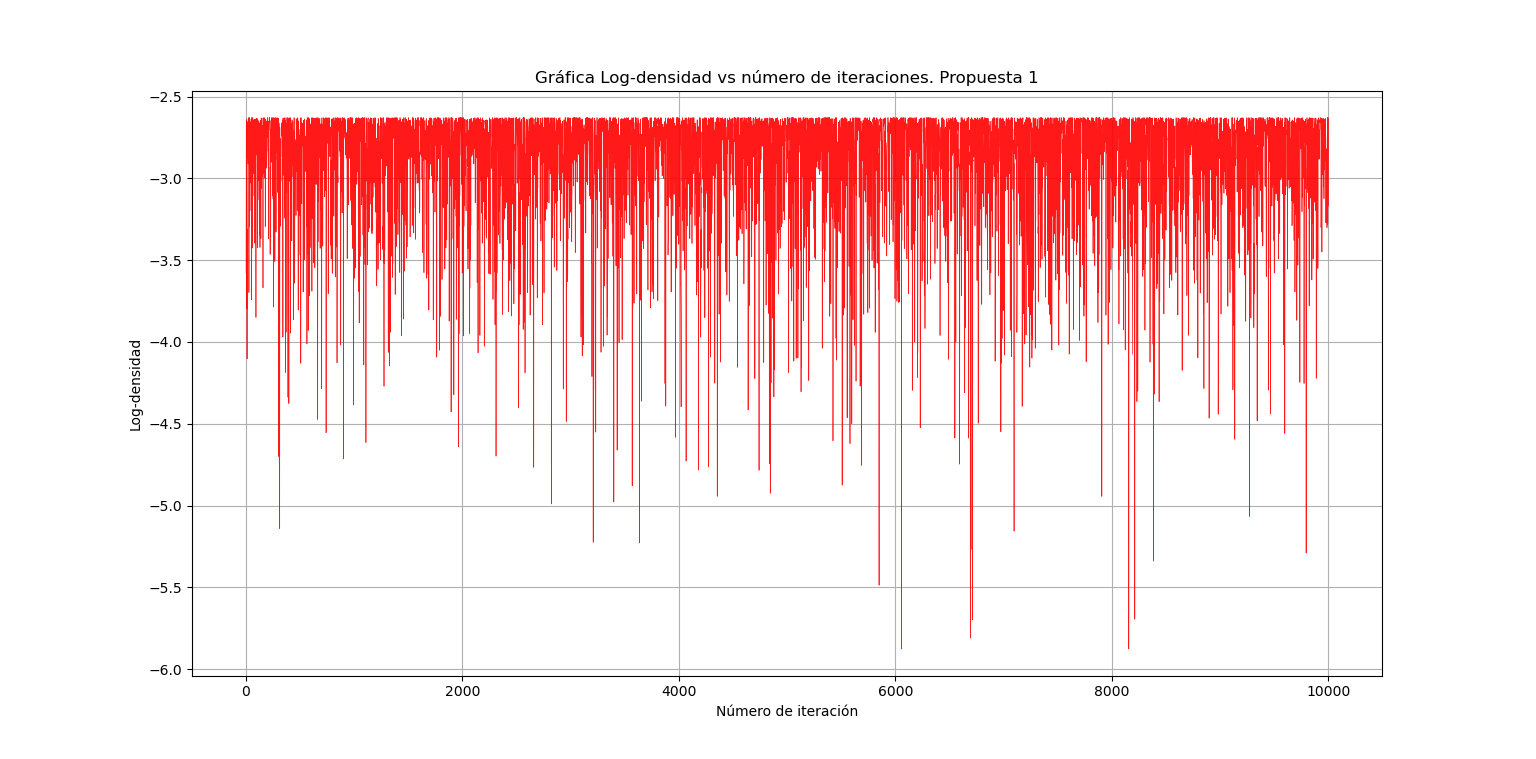
\includegraphics[width=\linewidth]{17.png}
        \caption{}
    \end{figure} 
    \begin{figure}[h!]
        \centering
        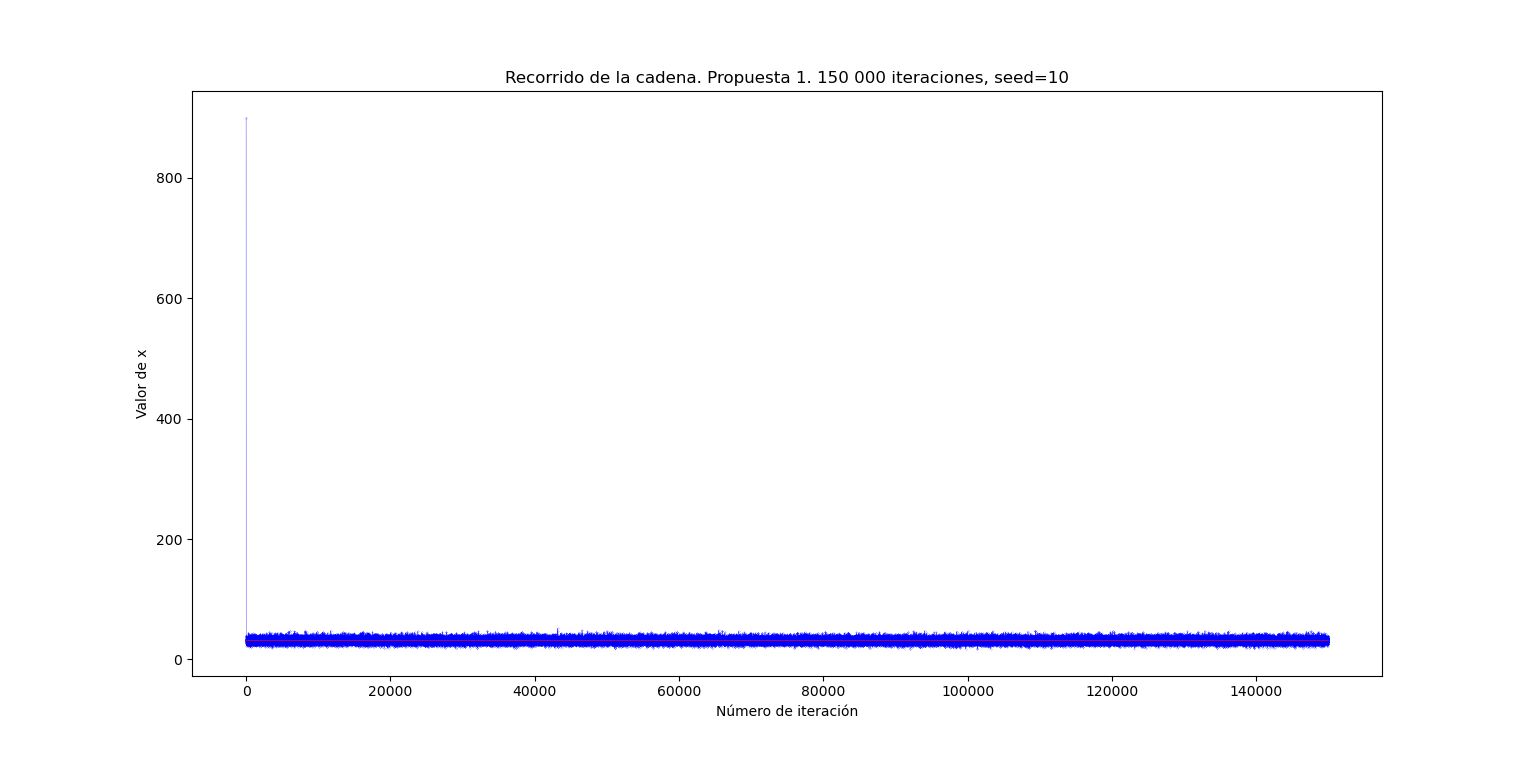
\includegraphics[width=\linewidth]{18.png}
        \caption{}
    \end{figure} 
    \begin{figure}[h!]
        \centering
        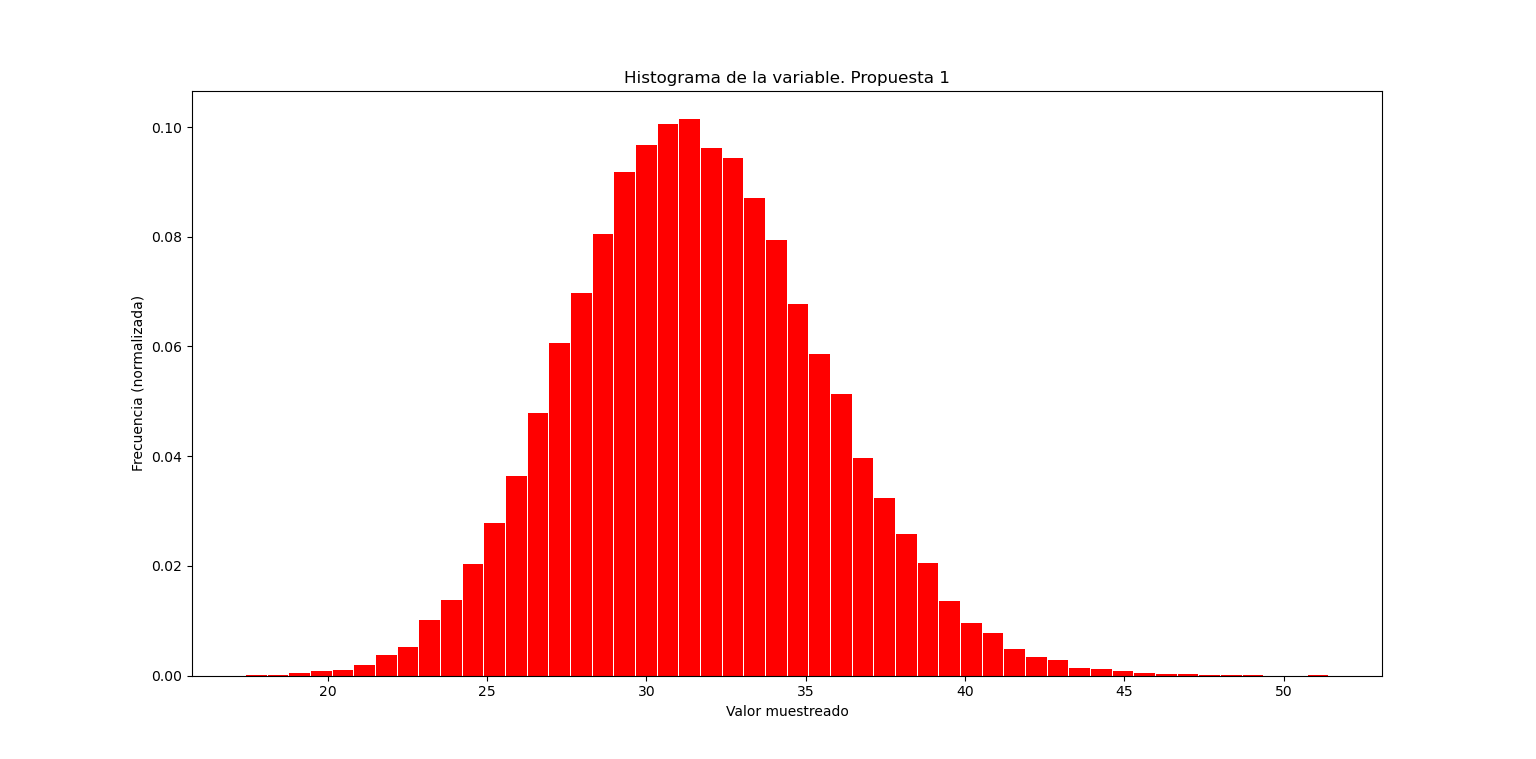
\includegraphics[width=\linewidth]{19.png}
        \caption{}
    \end{figure} 
    De la figura 17, se puede deducir que no hay un valor de burn-in que sea mejor a primera vista, por lo que 
    se decide tomar un burn-in genérico de 1000. En la figura 18 se puede apreciar que rápidamente se llega a muestreos cercanos 
    a la distribución objetivo. El histograma ya contempla el burn-in. Se puede apreciar una forma de densidad gamma con media en aproximadamente 31.415.\\

    Finalmente, se extrae la media de esta implementación, la cual se espera que esté próxima a $10\pi\approx31.1415926535$. La media extraída es de 31.59511788242531, que forma un 
    valor bastante cercano al real. \\

    Ahora bien, para el caso en el que se da otra propuesta, se selecciona a la propuesta $\Gamma(x,1)$, donde $x$ es el valor del punto actual de la cadena. Es decir, es 
    una propuesta que depende del punto en el que encontramos, a diferencia de la propuesta anterior en donde sin importar el punto inicial de la cadena, nuestra propuesta 
    directamente era el piso de $\alpha$, propuesta que directamente nos lleva tan solo en 1 paso (si hay aceptación a la primera) muy cerca de la distribución objetivo $\Gamma(\alpha,1)$.
    \\

    Con esta propuesta, se obtienen los siguientes resultados:
    \begin{figure}[h!]
        \centering
        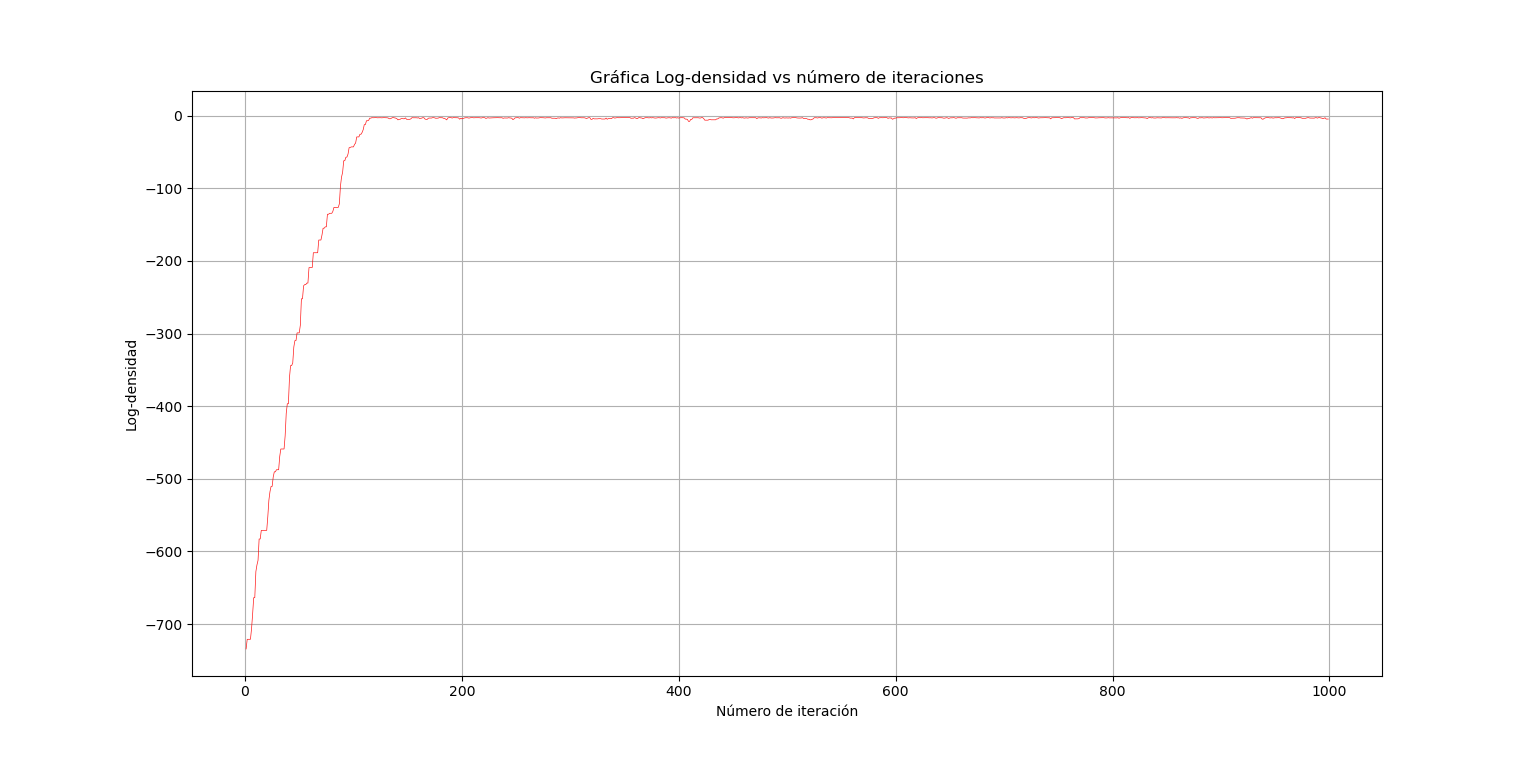
\includegraphics[width=\linewidth]{20.png}
        \caption{}
    \end{figure} 
    \begin{figure}[h!]
        \centering
        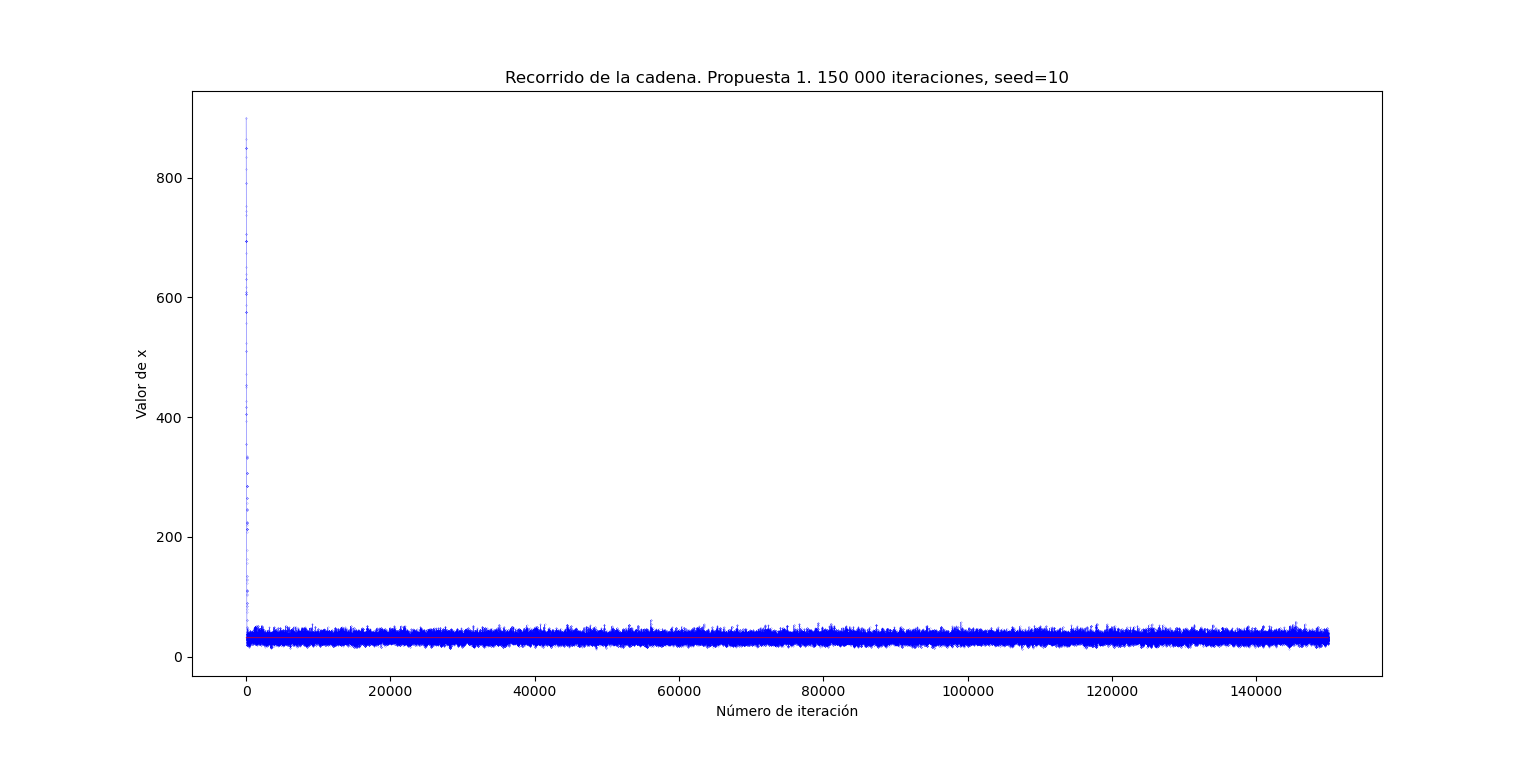
\includegraphics[width=\linewidth]{21.png}
        \caption{}
    \end{figure} 
    \begin{figure}[h!]
        \centering
        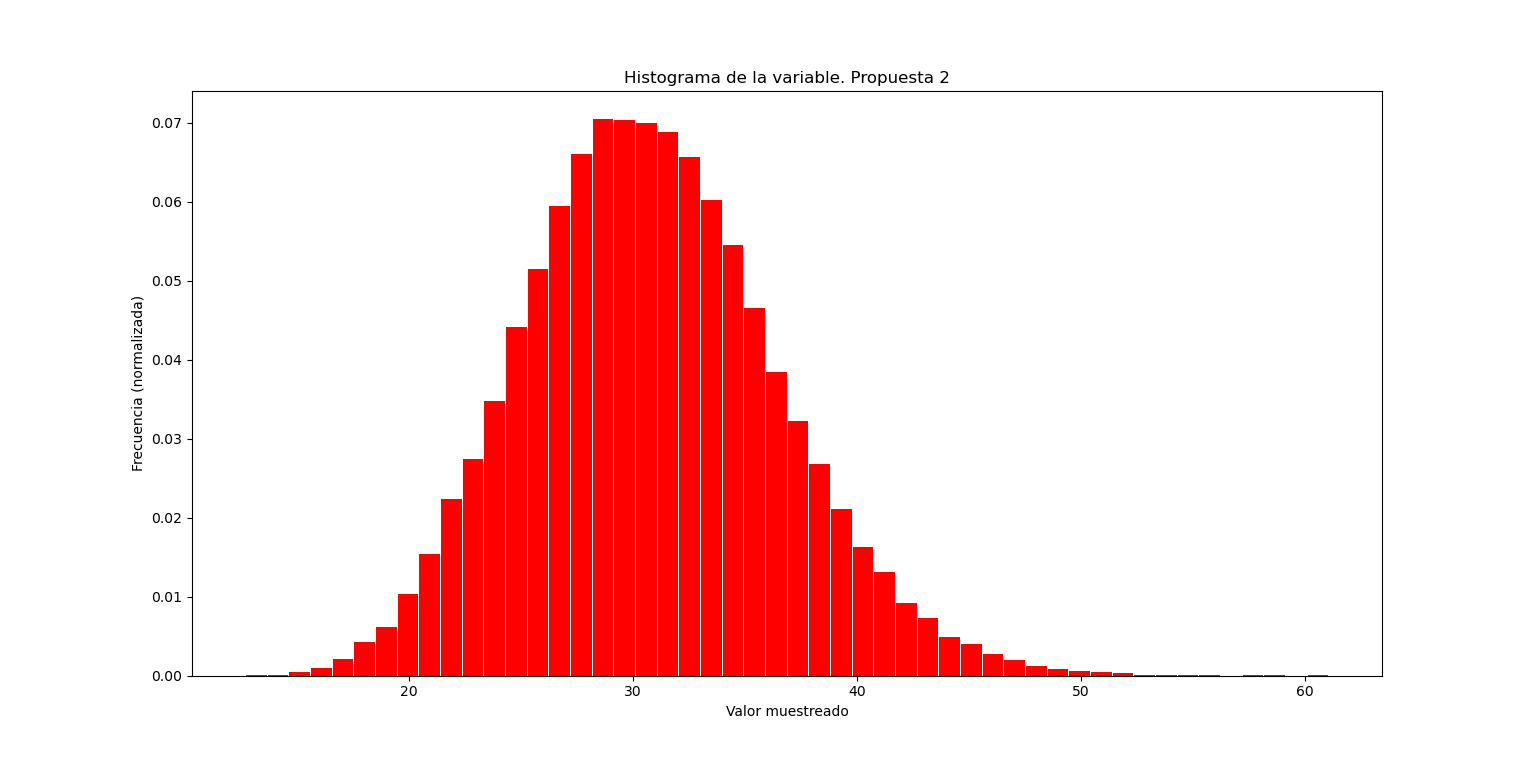
\includegraphics[width=\linewidth]{22.png}
        \caption{}
    \end{figure} 
    De la figura 20, se observa que un valor adecuado de burn-in ronda los 200. Sin embargo, aprovechando el tamaño d emuestra, se toma 
    el valor 1000 como burn-in. Como podemos observar de las figuras 21 y 22, la cadena avanza rápidamente a la distribución buscada, del histograma 
    se deduce que la muestra es buena. Finalmente se obtienen la media de los datos utilizando esta observación. Dicho valor es de $30.788501638194965$, que
    ciertamente se aleja más que el valor obtenido con la propuesta 1, pero no demasiado.\\

    Los detalles pedidos en esta implementación se resumen a continuación:
    \begin{itemize}
        \item \textbf{Distribución inicial}: tomamos el punto $X_0=900$ como propuesta inicial. Es sencillo tomar en este caso esa propuesta inicial
        lo cual nos ahora de paso el experimento que se pide en el ejercicio.
        \item \textbf{Grafica la evolución de la cadena}: ver figuras arriba.
        \item \textbf{Burn-in}: para ambos casos, se toma un burn-in=1000.
        \item \textbf{¿Qué tan eficiente es la cadena?}: sin duda la propuesta 1 tiene mejor desempeño, puesto que dicha propuesta 
        es independiente del punto en el que la cadena se encuentre. De hecho, el muestreo del valor siguiente se da de manera independiente, 
        por lo que es esperable que esta propuesta a diferencia de la propuesta 2, tenga mejores resultados.
        \\

        Una manera de cuantificar esto es con la gráfica de la log-densidad vs iteración. En la propuesta 1 no hay 
        evidencia de un burn-in, como se esperaría, mientras que en la propuesta 2 claro que la hay, ya que 
        la cadena debe avanzar desde el punto $\alpha=900$ hasta el punto $\alpha=31.41592...$.
    \end{itemize}
    \newpage

\section*{Ejercicio 3:}
Implementar Random Walk Metrópolis Hastings (RWMH) donde la distribución
    objetivo es $\mathcal{N}_2(\mu,\Sigma)$, con 
    \[
    \mu=\begin{pmatrix}
        3\\
        5
    \end{pmatrix} \ \text{ y } \ 
    \begin{pmatrix}
        1 & 0.9\\
        0.9 & 1
    \end{pmatrix}.    
    \]
    Utilizar como propuesta $\varepsilon_t\sim \mathcal{N}_2(\textbf{0},\sigma I)$. ¿Cómo elegir 
    $\sigma$ para que la cadena sea eficiente? ¿Qué consecuencias tiene la elección de $\sigma$?

    Como experimento, elige como punto inicial $x_0= \begin{pmatrix}
        1000\\
        1
    \end{pmatrix}$ y comenta los resultados.\\
    \subsection*{Solución:}
    Aquí realizamos la implementación de la cadena, primero con la propuesta de la tarea. Esto nos arroja los siguientes resultados:
    \begin{figure}[h!]
        \centering
        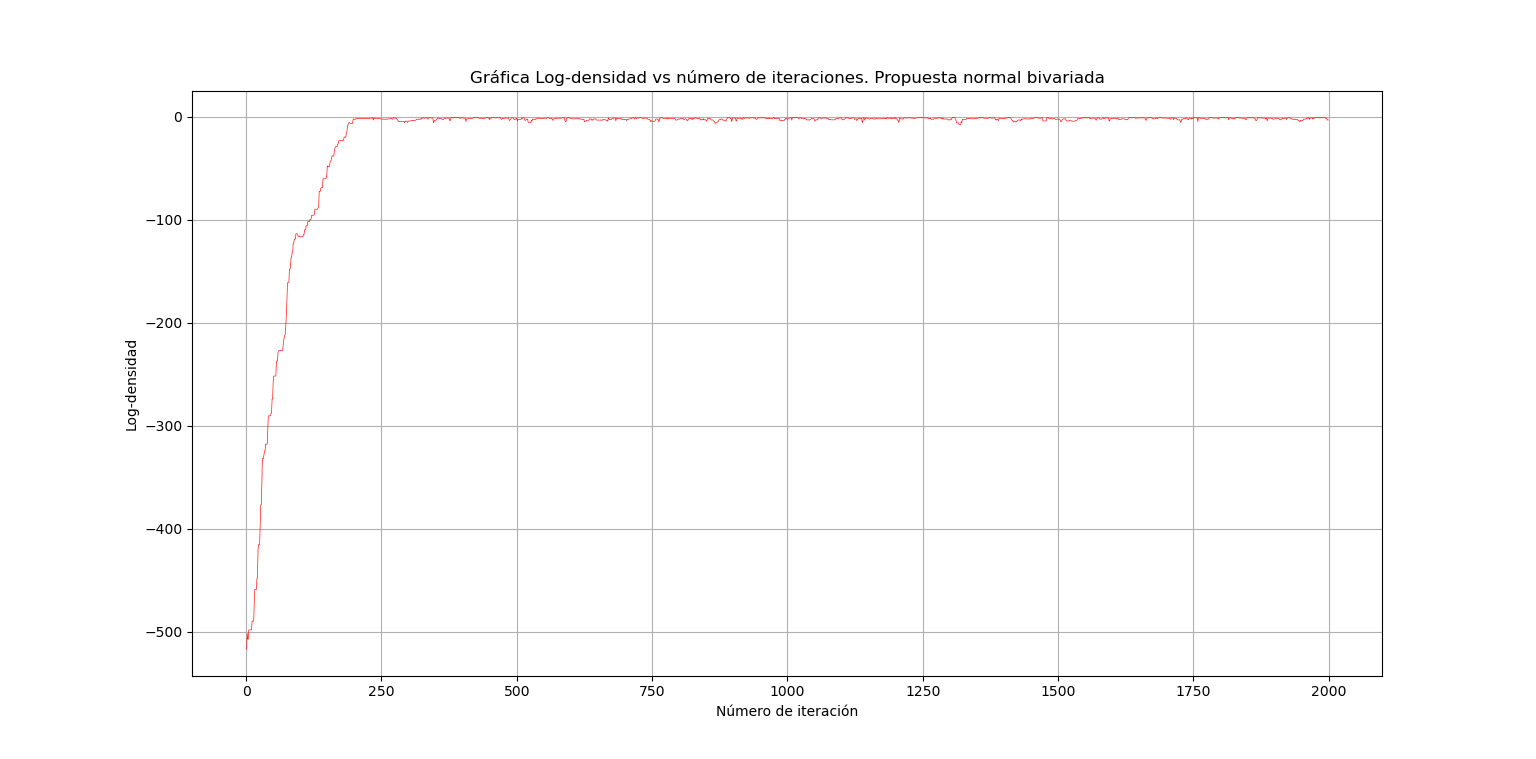
\includegraphics[width=\linewidth]{23.png}
        \caption{}
    \end{figure} 
    \begin{figure}[h!]
        \centering
        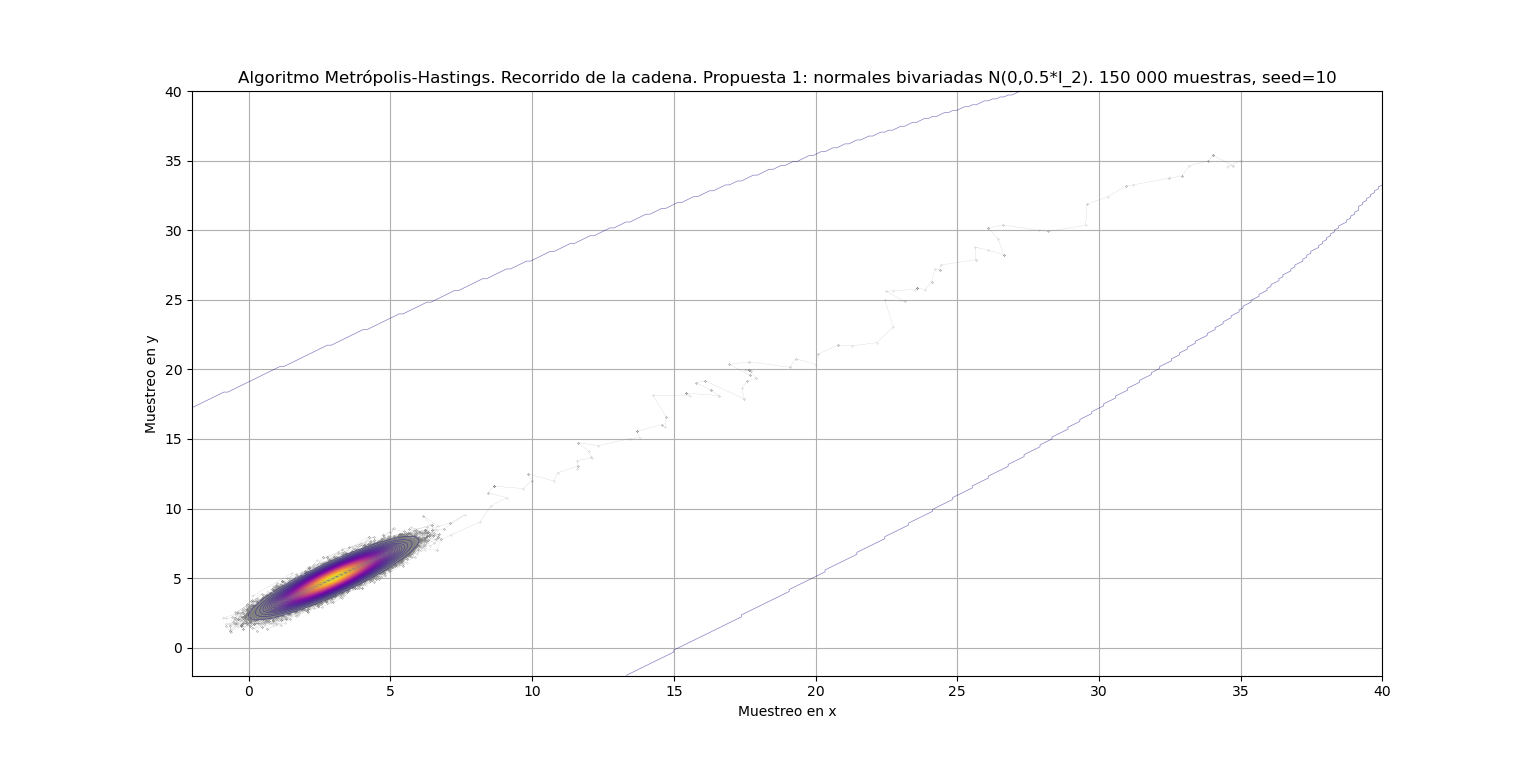
\includegraphics[width=\linewidth]{24.png}
        \caption{}
    \end{figure} 
    \begin{figure}[h!]
        \centering
        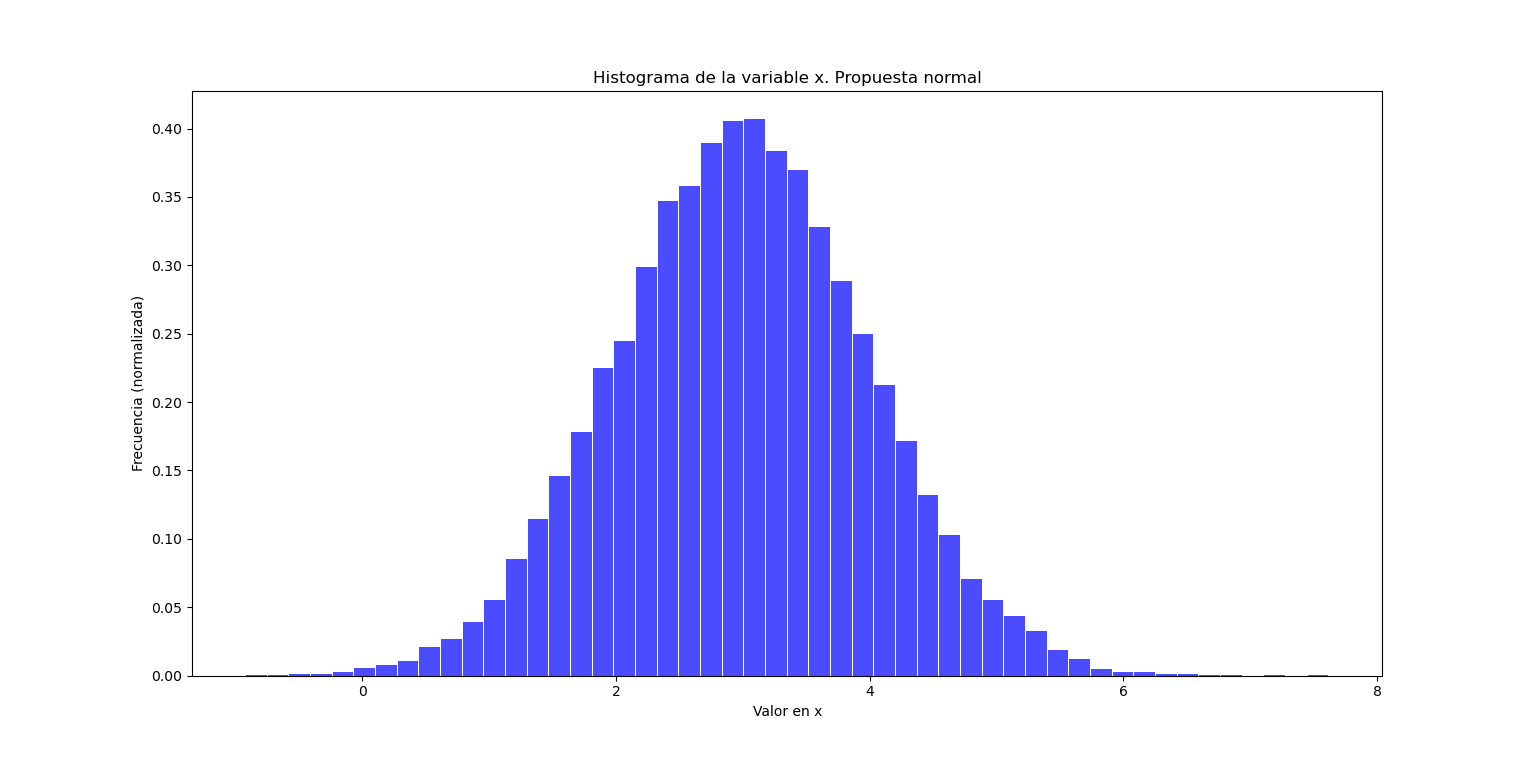
\includegraphics[width=\linewidth]{25.png}
        \caption{}
    \end{figure} 
    \begin{figure}[h!]
        \centering
        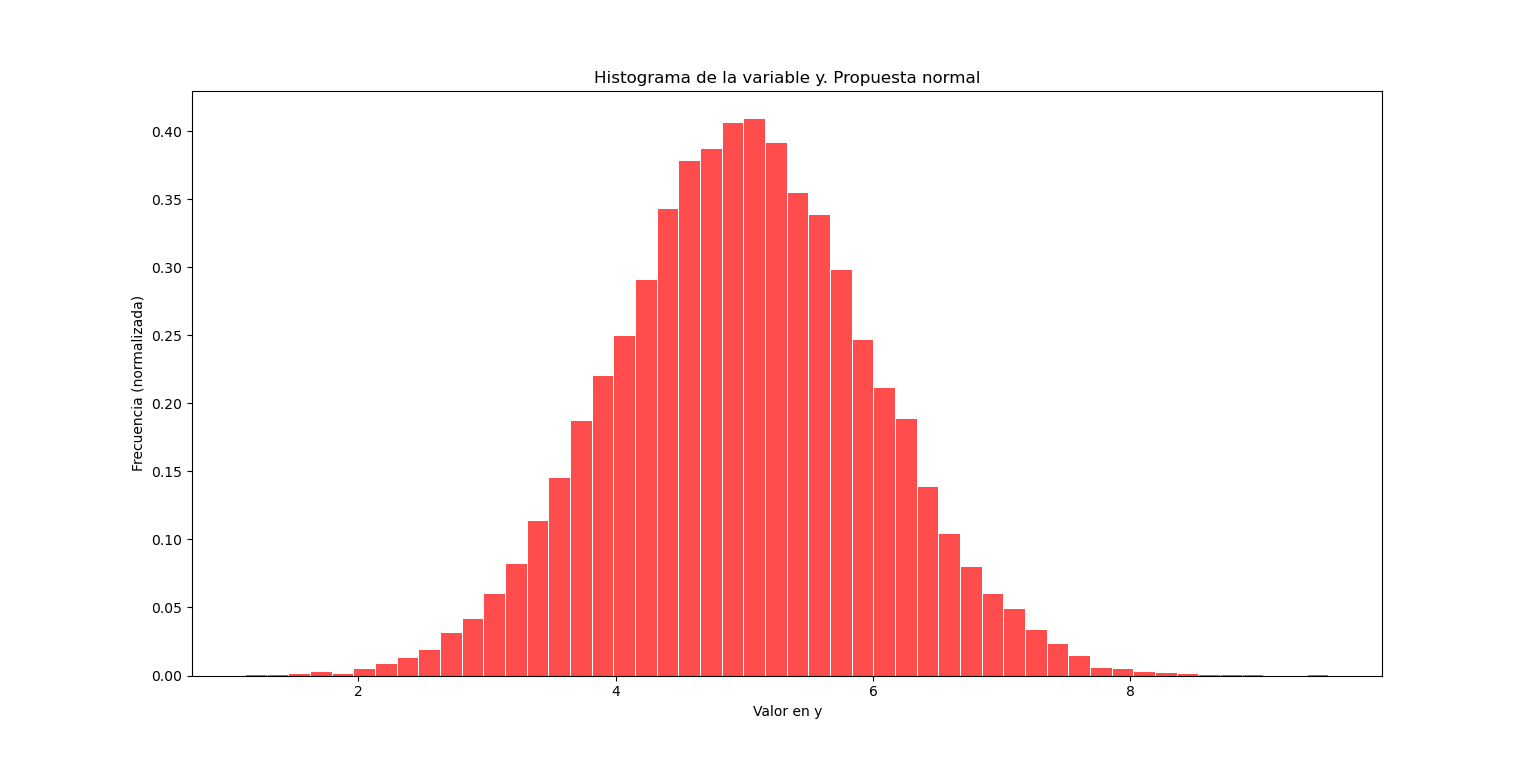
\includegraphics[width=\linewidth]{26.png}
        \caption{}
    \end{figure} 
    De la figura 23, apreciamos un valor de burn-in adecuado dado por 250. Sin embargo aprovechando el tamaño del muestreo, decidimos 
    tomar un burn-in de tamaño 2000. En la figura 24 se aprecia el camino desde el punto inicial, que en este caso se selecciona como $(35,35)$, hacia 
    la distribución objetivo. Las figuras 25 y 26 nos arrojan un histograma de variables que se parecen a las 
    densidades de dos normales centradas en 3 y 5, respectivamente, y varianza 1. Tal y como se espera.\\

    Finalmente, para la propuesta distinta, se selecciona una propuesta similar a la normal: una distribución $t$ de student 2-variada. De dicha implementación se obtiene 
    lo siguiente:

    \begin{figure}[h!]
        \centering
        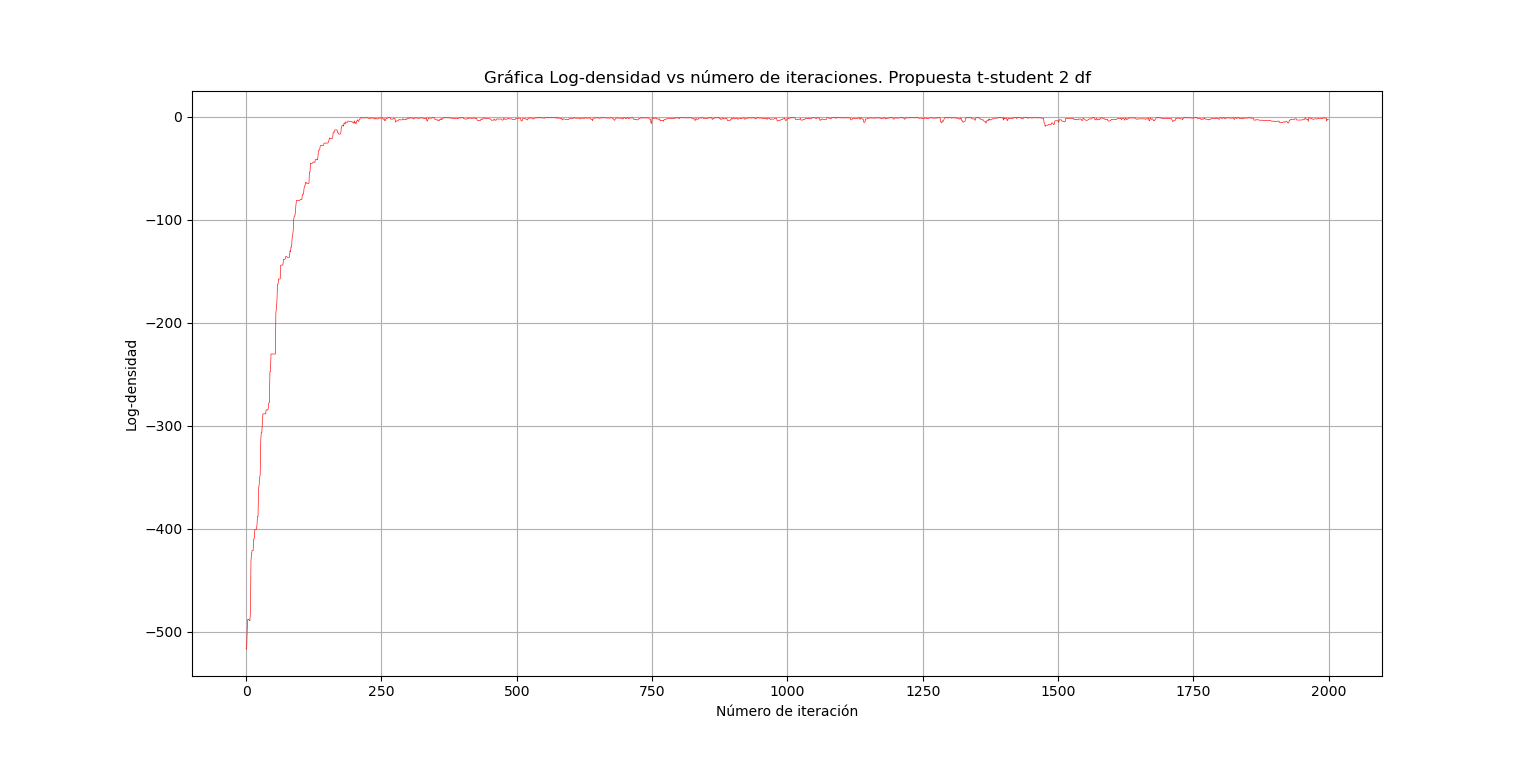
\includegraphics[width=\linewidth]{27.png}
        \caption{}
    \end{figure} 
    \begin{figure}[h!]
        \centering
        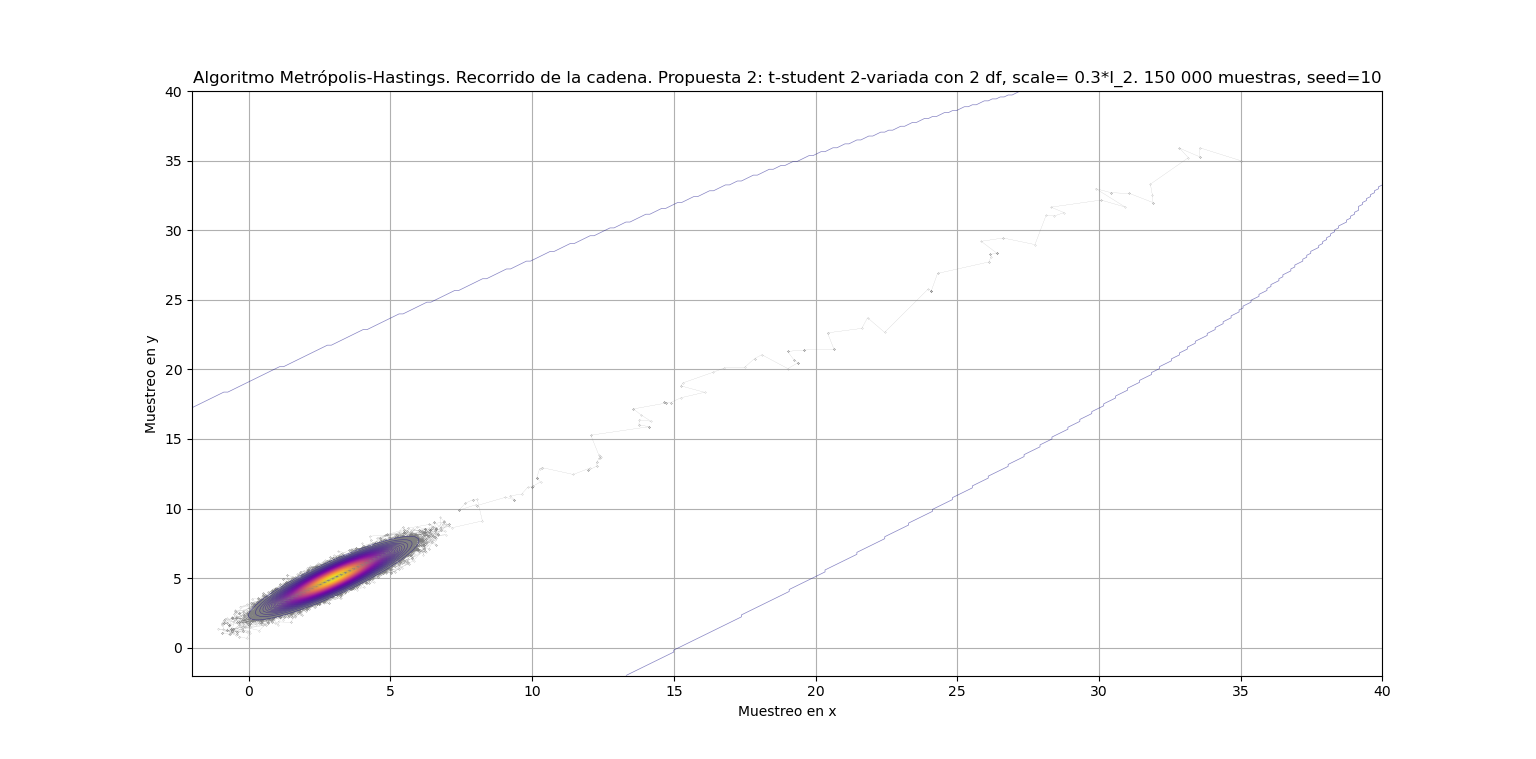
\includegraphics[width=\linewidth]{28.png}
        \caption{}
    \end{figure} 
    \begin{figure}[h!]
        \centering
        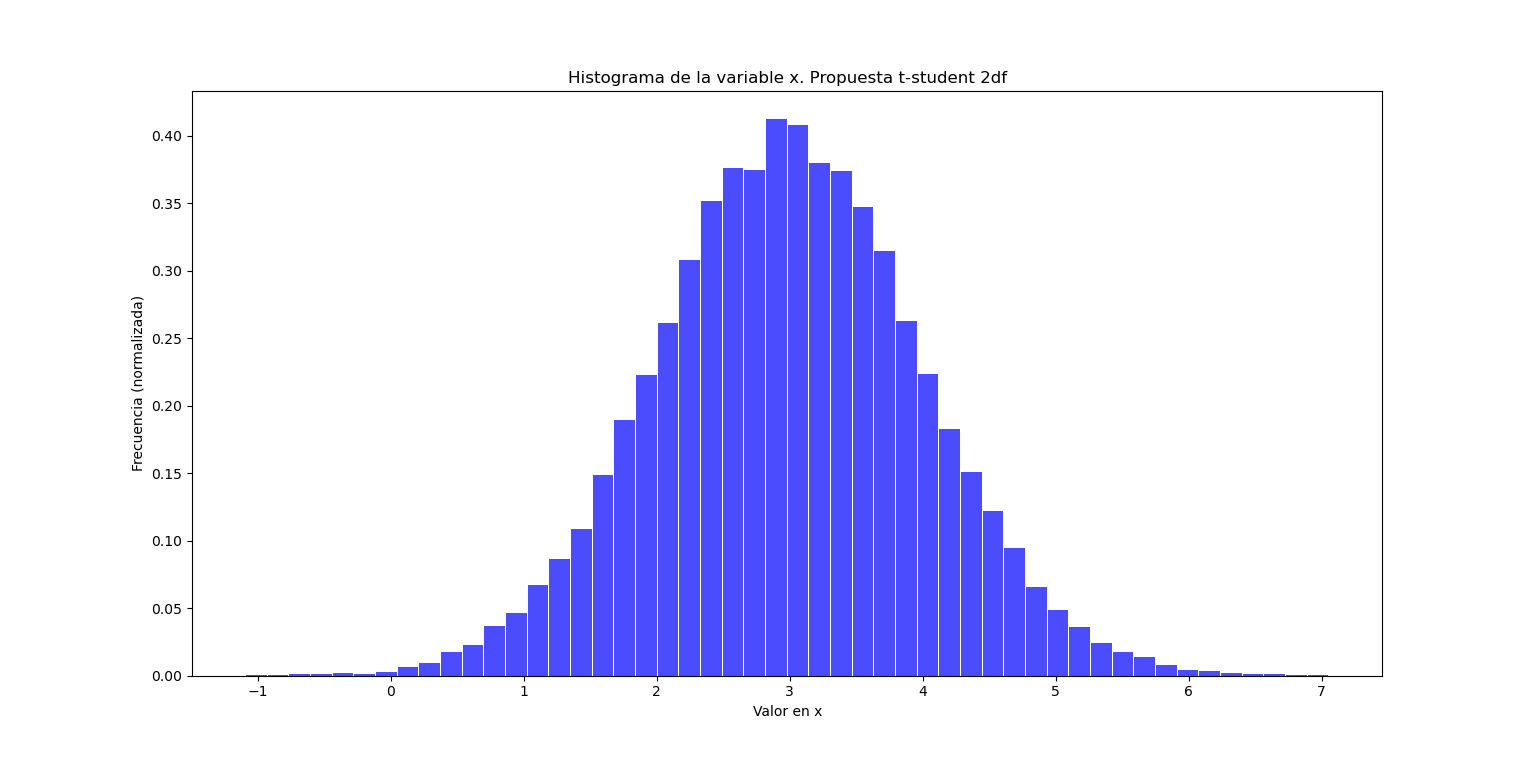
\includegraphics[width=\linewidth]{29.png}
        \caption{}
    \end{figure} 
    \begin{figure}[h!]
        \centering
        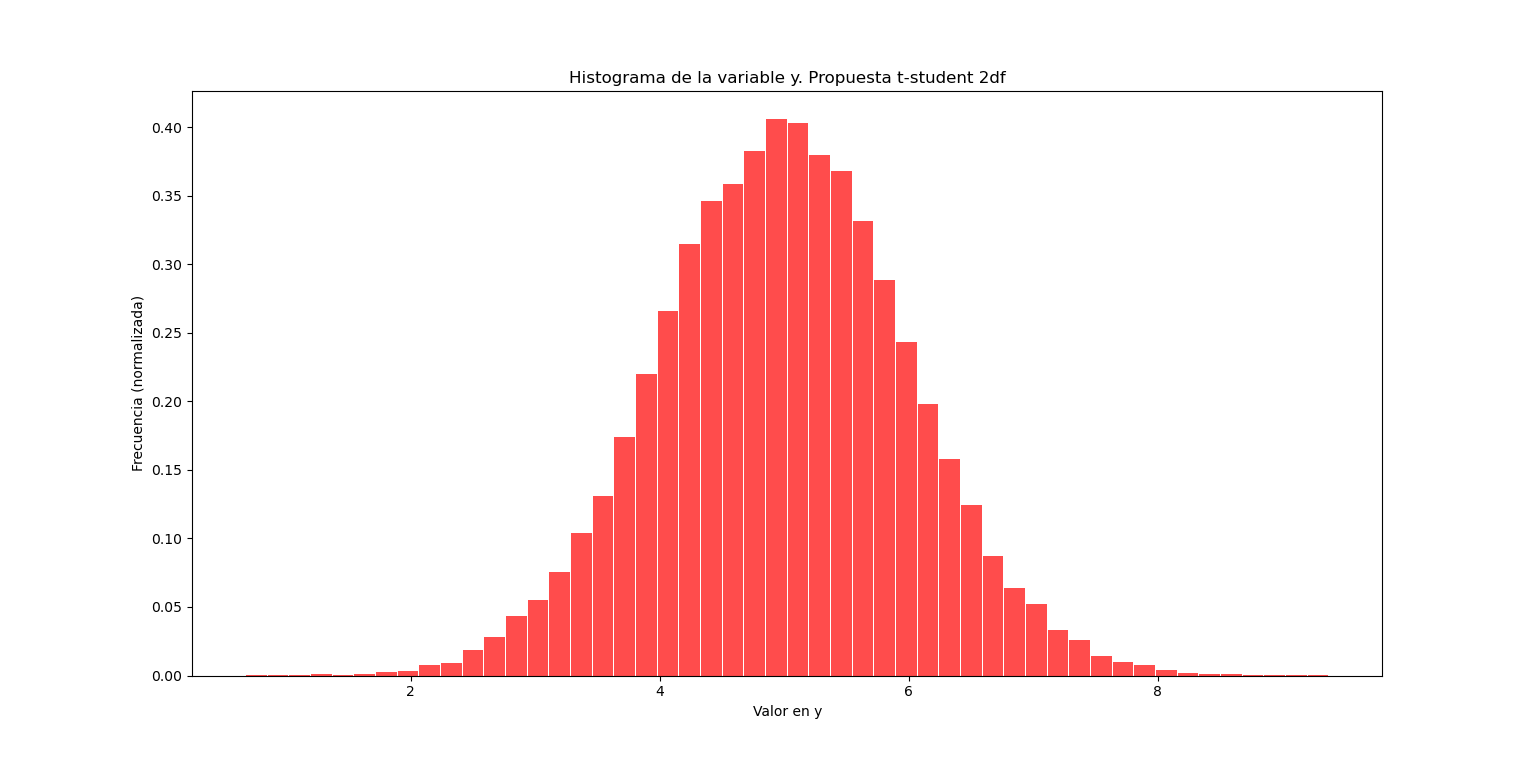
\includegraphics[width=\linewidth]{30.png}
        \caption{}
    \end{figure} 
    De la figura  27, el burn-in adecuado parece estar cerca del valor 250. Pero por simplicidad, nuevamente aprovechamos 
    el tamaño grande de la muestra y utilizamos burn-in=1000. En la figura 28 se aprecia el recorrido de la cadena. A diferencia de lo que  sucede 
    con la propuesta normal, el avance con la propuesta $t$ de student multivariada, es más rápido en ciertos momentos que con el de la normal.
    Los histogramas de las figuras 29 y 30 nuevamente presentan un buen comportamiento. Son similares a las normales 
    de media 3 y varianza 1, y de media 5 y varianza 1, respectivamente en cada coordenada.\\
    
    Se detalla a continuación lo pedido:
    \begin{itemize}
        \item \textbf{Distribución inicial}: tomamos el vector $X_0=(35,35)$ como propuesta inicial en ambos casos.
        \item \textbf{Grafica la evolución de la cadena}: ver figuras arriba.
        \item \textbf{Burn-in}: para ambos casos, se toma un burn-in=1000.
        \item \textbf{¿Qué tan eficiente es la cadena?}: a simple vista el desempeño de la cadena parece ser bueno. El burn-in en ambos es pequeño, del orden 
        de 250, similar en ambos casos, por lo que parece ser que ambas propuestas son buenas.

        Cabe mencionar que la matriz de covarianzas, así como el parámetro de escala para la t 2-variada, están dadas por 
        \[
        \begin{pmatrix}
            0.5 & 0\\
            0 & 0.5
        \end{pmatrix},    
        \]
        esto es, $\sigma=0.5$ es el parámetro usado.
    \end{itemize}
    Finalmente, se realiza el experimento mencionado. Seleccionamos el punto $X_0=(1000,1)$ como punto inicial. Nótese que la cadena no salta con un punto inicial tan 
    lejano, como se puede ver en la siguiente figura 31.

    \begin{figure}[h!]
        \centering
        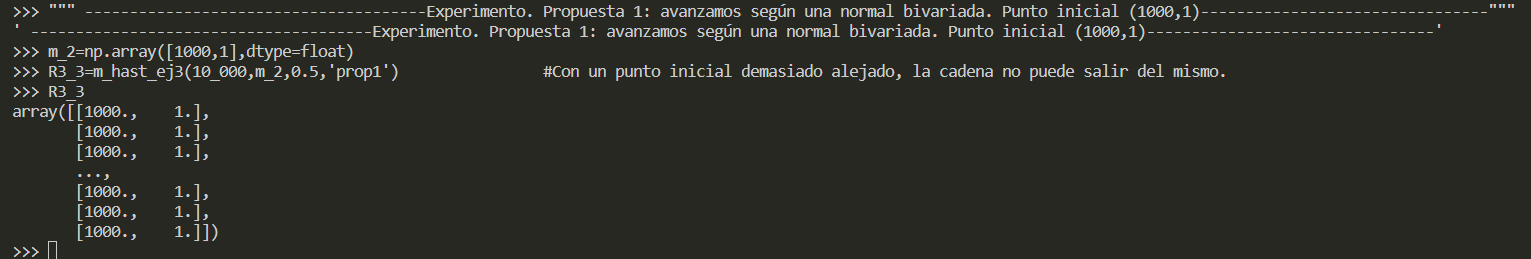
\includegraphics[width=\linewidth]{31.png}
        \caption{}
    \end{figure} 
    Esto nos recuerda que la selección de un punto adecuado de inicio es importante también para el correcto muestreo de la distribución 
    objetivo usando Metropolis-Hastings.

\end{document}  